% Options for packages loaded elsewhere
\PassOptionsToPackage{unicode}{hyperref}
\PassOptionsToPackage{hyphens}{url}
\PassOptionsToPackage{dvipsnames,svgnames,x11names}{xcolor}
%
\documentclass[
  letterpaper,
  DIV=11,
  numbers=noendperiod]{scrreprt}

\usepackage{amsmath,amssymb}
\usepackage{iftex}
\ifPDFTeX
  \usepackage[T1]{fontenc}
  \usepackage[utf8]{inputenc}
  \usepackage{textcomp} % provide euro and other symbols
\else % if luatex or xetex
  \usepackage{unicode-math}
  \defaultfontfeatures{Scale=MatchLowercase}
  \defaultfontfeatures[\rmfamily]{Ligatures=TeX,Scale=1}
\fi
\usepackage{lmodern}
\ifPDFTeX\else  
    % xetex/luatex font selection
\fi
% Use upquote if available, for straight quotes in verbatim environments
\IfFileExists{upquote.sty}{\usepackage{upquote}}{}
\IfFileExists{microtype.sty}{% use microtype if available
  \usepackage[]{microtype}
  \UseMicrotypeSet[protrusion]{basicmath} % disable protrusion for tt fonts
}{}
\makeatletter
\@ifundefined{KOMAClassName}{% if non-KOMA class
  \IfFileExists{parskip.sty}{%
    \usepackage{parskip}
  }{% else
    \setlength{\parindent}{0pt}
    \setlength{\parskip}{6pt plus 2pt minus 1pt}}
}{% if KOMA class
  \KOMAoptions{parskip=half}}
\makeatother
\usepackage{xcolor}
\setlength{\emergencystretch}{3em} % prevent overfull lines
\setcounter{secnumdepth}{5}
% Make \paragraph and \subparagraph free-standing
\makeatletter
\ifx\paragraph\undefined\else
  \let\oldparagraph\paragraph
  \renewcommand{\paragraph}{
    \@ifstar
      \xxxParagraphStar
      \xxxParagraphNoStar
  }
  \newcommand{\xxxParagraphStar}[1]{\oldparagraph*{#1}\mbox{}}
  \newcommand{\xxxParagraphNoStar}[1]{\oldparagraph{#1}\mbox{}}
\fi
\ifx\subparagraph\undefined\else
  \let\oldsubparagraph\subparagraph
  \renewcommand{\subparagraph}{
    \@ifstar
      \xxxSubParagraphStar
      \xxxSubParagraphNoStar
  }
  \newcommand{\xxxSubParagraphStar}[1]{\oldsubparagraph*{#1}\mbox{}}
  \newcommand{\xxxSubParagraphNoStar}[1]{\oldsubparagraph{#1}\mbox{}}
\fi
\makeatother

\usepackage{color}
\usepackage{fancyvrb}
\newcommand{\VerbBar}{|}
\newcommand{\VERB}{\Verb[commandchars=\\\{\}]}
\DefineVerbatimEnvironment{Highlighting}{Verbatim}{commandchars=\\\{\}}
% Add ',fontsize=\small' for more characters per line
\usepackage{framed}
\definecolor{shadecolor}{RGB}{241,243,245}
\newenvironment{Shaded}{\begin{snugshade}}{\end{snugshade}}
\newcommand{\AlertTok}[1]{\textcolor[rgb]{0.68,0.00,0.00}{#1}}
\newcommand{\AnnotationTok}[1]{\textcolor[rgb]{0.37,0.37,0.37}{#1}}
\newcommand{\AttributeTok}[1]{\textcolor[rgb]{0.40,0.45,0.13}{#1}}
\newcommand{\BaseNTok}[1]{\textcolor[rgb]{0.68,0.00,0.00}{#1}}
\newcommand{\BuiltInTok}[1]{\textcolor[rgb]{0.00,0.23,0.31}{#1}}
\newcommand{\CharTok}[1]{\textcolor[rgb]{0.13,0.47,0.30}{#1}}
\newcommand{\CommentTok}[1]{\textcolor[rgb]{0.37,0.37,0.37}{#1}}
\newcommand{\CommentVarTok}[1]{\textcolor[rgb]{0.37,0.37,0.37}{\textit{#1}}}
\newcommand{\ConstantTok}[1]{\textcolor[rgb]{0.56,0.35,0.01}{#1}}
\newcommand{\ControlFlowTok}[1]{\textcolor[rgb]{0.00,0.23,0.31}{\textbf{#1}}}
\newcommand{\DataTypeTok}[1]{\textcolor[rgb]{0.68,0.00,0.00}{#1}}
\newcommand{\DecValTok}[1]{\textcolor[rgb]{0.68,0.00,0.00}{#1}}
\newcommand{\DocumentationTok}[1]{\textcolor[rgb]{0.37,0.37,0.37}{\textit{#1}}}
\newcommand{\ErrorTok}[1]{\textcolor[rgb]{0.68,0.00,0.00}{#1}}
\newcommand{\ExtensionTok}[1]{\textcolor[rgb]{0.00,0.23,0.31}{#1}}
\newcommand{\FloatTok}[1]{\textcolor[rgb]{0.68,0.00,0.00}{#1}}
\newcommand{\FunctionTok}[1]{\textcolor[rgb]{0.28,0.35,0.67}{#1}}
\newcommand{\ImportTok}[1]{\textcolor[rgb]{0.00,0.46,0.62}{#1}}
\newcommand{\InformationTok}[1]{\textcolor[rgb]{0.37,0.37,0.37}{#1}}
\newcommand{\KeywordTok}[1]{\textcolor[rgb]{0.00,0.23,0.31}{\textbf{#1}}}
\newcommand{\NormalTok}[1]{\textcolor[rgb]{0.00,0.23,0.31}{#1}}
\newcommand{\OperatorTok}[1]{\textcolor[rgb]{0.37,0.37,0.37}{#1}}
\newcommand{\OtherTok}[1]{\textcolor[rgb]{0.00,0.23,0.31}{#1}}
\newcommand{\PreprocessorTok}[1]{\textcolor[rgb]{0.68,0.00,0.00}{#1}}
\newcommand{\RegionMarkerTok}[1]{\textcolor[rgb]{0.00,0.23,0.31}{#1}}
\newcommand{\SpecialCharTok}[1]{\textcolor[rgb]{0.37,0.37,0.37}{#1}}
\newcommand{\SpecialStringTok}[1]{\textcolor[rgb]{0.13,0.47,0.30}{#1}}
\newcommand{\StringTok}[1]{\textcolor[rgb]{0.13,0.47,0.30}{#1}}
\newcommand{\VariableTok}[1]{\textcolor[rgb]{0.07,0.07,0.07}{#1}}
\newcommand{\VerbatimStringTok}[1]{\textcolor[rgb]{0.13,0.47,0.30}{#1}}
\newcommand{\WarningTok}[1]{\textcolor[rgb]{0.37,0.37,0.37}{\textit{#1}}}

\providecommand{\tightlist}{%
  \setlength{\itemsep}{0pt}\setlength{\parskip}{0pt}}\usepackage{longtable,booktabs,array}
\usepackage{calc} % for calculating minipage widths
% Correct order of tables after \paragraph or \subparagraph
\usepackage{etoolbox}
\makeatletter
\patchcmd\longtable{\par}{\if@noskipsec\mbox{}\fi\par}{}{}
\makeatother
% Allow footnotes in longtable head/foot
\IfFileExists{footnotehyper.sty}{\usepackage{footnotehyper}}{\usepackage{footnote}}
\makesavenoteenv{longtable}
\usepackage{graphicx}
\makeatletter
\def\maxwidth{\ifdim\Gin@nat@width>\linewidth\linewidth\else\Gin@nat@width\fi}
\def\maxheight{\ifdim\Gin@nat@height>\textheight\textheight\else\Gin@nat@height\fi}
\makeatother
% Scale images if necessary, so that they will not overflow the page
% margins by default, and it is still possible to overwrite the defaults
% using explicit options in \includegraphics[width, height, ...]{}
\setkeys{Gin}{width=\maxwidth,height=\maxheight,keepaspectratio}
% Set default figure placement to htbp
\makeatletter
\def\fps@figure{htbp}
\makeatother
% definitions for citeproc citations
\NewDocumentCommand\citeproctext{}{}
\NewDocumentCommand\citeproc{mm}{%
  \begingroup\def\citeproctext{#2}\cite{#1}\endgroup}
\makeatletter
 % allow citations to break across lines
 \let\@cite@ofmt\@firstofone
 % avoid brackets around text for \cite:
 \def\@biblabel#1{}
 \def\@cite#1#2{{#1\if@tempswa , #2\fi}}
\makeatother
\newlength{\cslhangindent}
\setlength{\cslhangindent}{1.5em}
\newlength{\csllabelwidth}
\setlength{\csllabelwidth}{3em}
\newenvironment{CSLReferences}[2] % #1 hanging-indent, #2 entry-spacing
 {\begin{list}{}{%
  \setlength{\itemindent}{0pt}
  \setlength{\leftmargin}{0pt}
  \setlength{\parsep}{0pt}
  % turn on hanging indent if param 1 is 1
  \ifodd #1
   \setlength{\leftmargin}{\cslhangindent}
   \setlength{\itemindent}{-1\cslhangindent}
  \fi
  % set entry spacing
  \setlength{\itemsep}{#2\baselineskip}}}
 {\end{list}}
\usepackage{calc}
\newcommand{\CSLBlock}[1]{\hfill\break\parbox[t]{\linewidth}{\strut\ignorespaces#1\strut}}
\newcommand{\CSLLeftMargin}[1]{\parbox[t]{\csllabelwidth}{\strut#1\strut}}
\newcommand{\CSLRightInline}[1]{\parbox[t]{\linewidth - \csllabelwidth}{\strut#1\strut}}
\newcommand{\CSLIndent}[1]{\hspace{\cslhangindent}#1}

\KOMAoption{captions}{tableheading}
\makeatletter
\@ifpackageloaded{bookmark}{}{\usepackage{bookmark}}
\makeatother
\makeatletter
\@ifpackageloaded{caption}{}{\usepackage{caption}}
\AtBeginDocument{%
\ifdefined\contentsname
  \renewcommand*\contentsname{Table of contents}
\else
  \newcommand\contentsname{Table of contents}
\fi
\ifdefined\listfigurename
  \renewcommand*\listfigurename{List of Figures}
\else
  \newcommand\listfigurename{List of Figures}
\fi
\ifdefined\listtablename
  \renewcommand*\listtablename{List of Tables}
\else
  \newcommand\listtablename{List of Tables}
\fi
\ifdefined\figurename
  \renewcommand*\figurename{Figure}
\else
  \newcommand\figurename{Figure}
\fi
\ifdefined\tablename
  \renewcommand*\tablename{Table}
\else
  \newcommand\tablename{Table}
\fi
}
\@ifpackageloaded{float}{}{\usepackage{float}}
\floatstyle{ruled}
\@ifundefined{c@chapter}{\newfloat{codelisting}{h}{lop}}{\newfloat{codelisting}{h}{lop}[chapter]}
\floatname{codelisting}{Listing}
\newcommand*\listoflistings{\listof{codelisting}{List of Listings}}
\makeatother
\makeatletter
\makeatother
\makeatletter
\@ifpackageloaded{caption}{}{\usepackage{caption}}
\@ifpackageloaded{subcaption}{}{\usepackage{subcaption}}
\makeatother

\ifLuaTeX
  \usepackage{selnolig}  % disable illegal ligatures
\fi
\usepackage{bookmark}

\IfFileExists{xurl.sty}{\usepackage{xurl}}{} % add URL line breaks if available
\urlstyle{same} % disable monospaced font for URLs
\hypersetup{
  pdftitle={Introdução aos modelos lineares dinâmicos},
  pdfauthor={James D Santos},
  colorlinks=true,
  linkcolor={blue},
  filecolor={Maroon},
  citecolor={Blue},
  urlcolor={Blue},
  pdfcreator={LaTeX via pandoc}}


\title{Introdução aos modelos lineares dinâmicos}
\author{James D Santos}
\date{2025-04-09}

\begin{document}
\maketitle

\renewcommand*\contentsname{Table of contents}
{
\hypersetup{linkcolor=}
\setcounter{tocdepth}{2}
\tableofcontents
}

\bookmarksetup{startatroot}

\chapter*{Prefácio}\label{prefuxe1cio}
\addcontentsline{toc}{chapter}{Prefácio}

\markboth{Prefácio}{Prefácio}

\bookmarksetup{startatroot}

\chapter{\texorpdfstring{Manipulação de séries temporais univariadas no
software
\texttt{R}}{Manipulação de séries temporais univariadas no software R}}\label{manipulauxe7uxe3o-de-suxe9ries-temporais-univariadas-no-software-r}

\section{Definição de séries
temporais}\label{definiuxe7uxe3o-de-suxe9ries-temporais}

Considere um fenômeno aleatório que é observado ao longo do tempo. A
coleção de variáveis aleatórias indexadas no tempo, associadas a este
fenômeno, é denominada série temporal. Neste caso, para cada instante de
tempo \(t\), há uma variável \(X(t)\) associada.

\begin{figure}[H]

{\centering 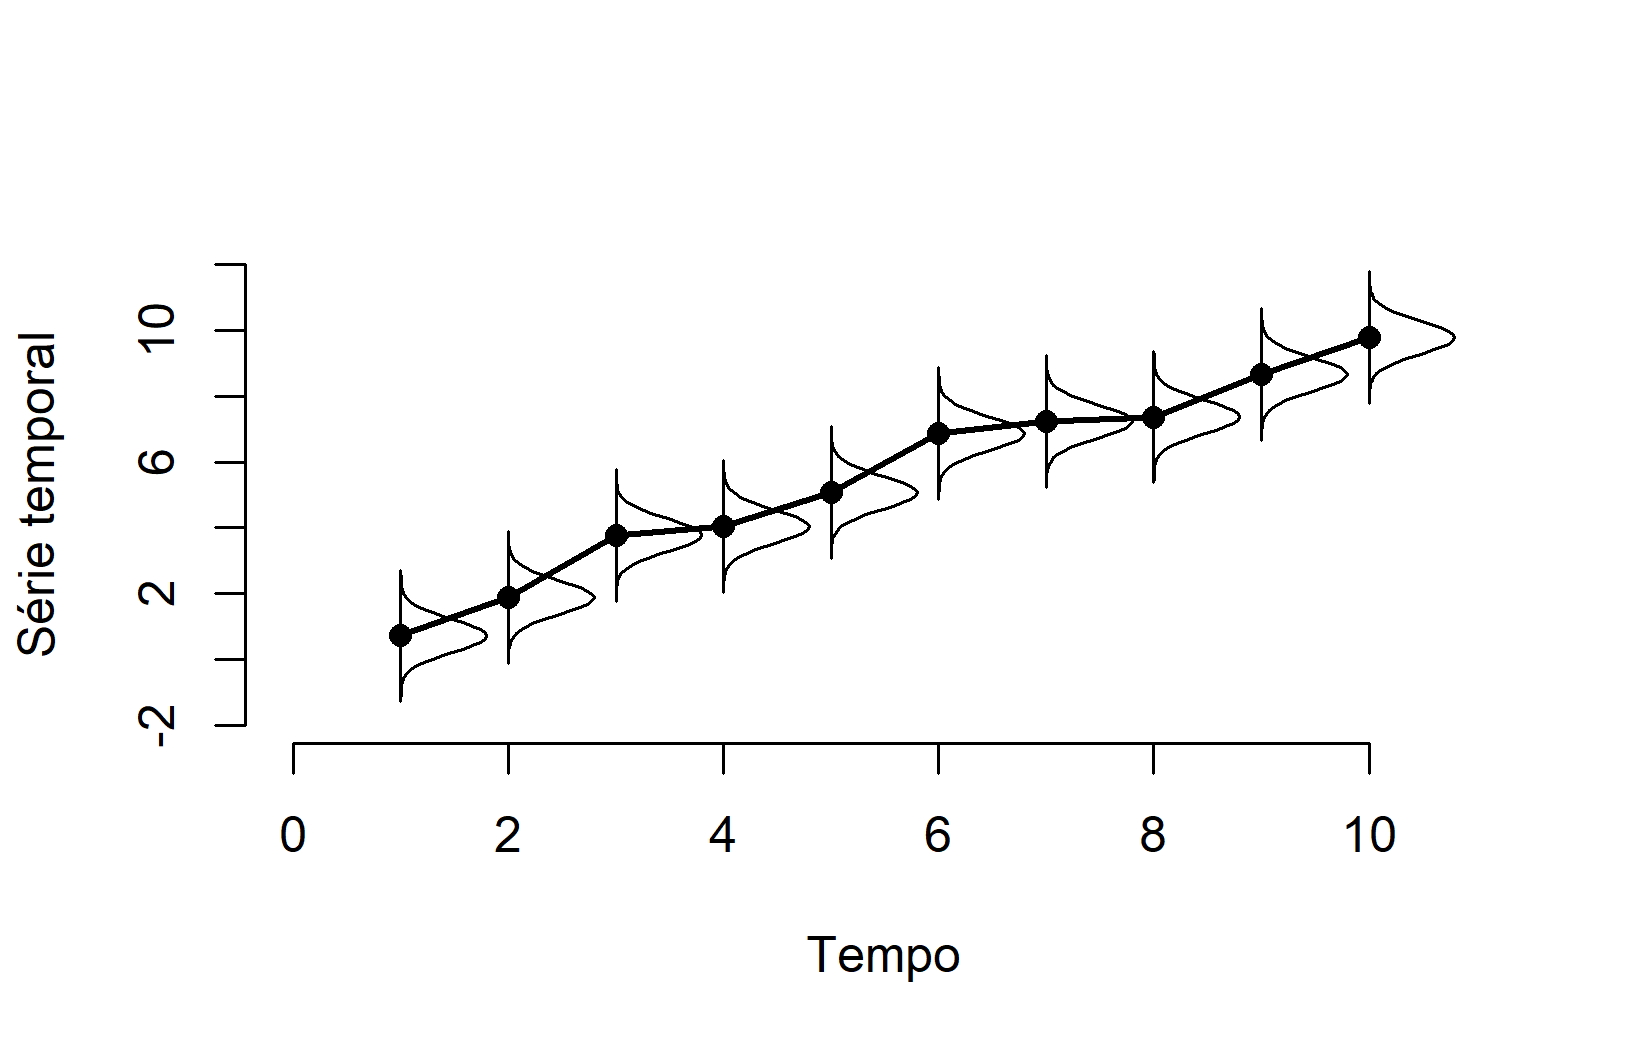
\includegraphics{intro_files/figure-pdf/figura1-1.png}

}

\caption{Figure 1 - Ilustração de uma série temporal}

\end{figure}%

Alguns autores definem séries temporais simplesmente como valores
observados ao longo do tempo.No entanto, essa definição não é útil para
nós, uma vez que o tempo não necessariamente possui influência na
variável, ou seja, é possível que a distribuição de \(X(t)\) não dependa
de \(t\).

Importante: estamos interessados apenas em séries temporais nas quais o
modelo de probabilidades depende do tempo \(t\).

A partir deste momento, \(X(t)\) será escrita como \(X_t\) e
representará a variável aleatória associada ao tempo \(t\) e a versão
minúscula \(x_t\) representará o valor observado.

\section{\texorpdfstring{A classe \texttt{ts} e a função
\texttt{window}}{A classe ts e a função window}}\label{a-classe-ts-e-a-funuxe7uxe3o-window}

Nessa seção vamos distutir a classe \texttt{ts} do \texttt{R}. Ela é
particularmente útil para fazer gráficos de séries temporais. A função
\texttt{ts} possui vários argumentos importantes:

\begin{itemize}
\item
  \texttt{data}: vetor ou matriz da série observada
\item
  \texttt{frequency}: esse valor representa o número de observações por
  período. Vamos discutir essa particularidade em outro momento, mas
  para a maioria das séries, o período é representado por um ano e o
  valor de \texttt{frequency} está relacionado com quantas observações
  são necessárias para completar um ano. Por exemplo, se os dados são
  registrados mensalmente, temos \texttt{frequency=12}. Em caso de
  trimestres, \texttt{frequency=4}. O valor padrão é
  \texttt{frequency=1}.
\item
  \texttt{deltat}: é o inverso do número de observações por período.
  Apenas um entre \texttt{frequency} e \texttt{deltat} deve ser dado.
\item
  \texttt{start}: representa o tempo no qual a série começa. Pode ser
  representado por um único número ou por um vetor de dois números, com
  o segundo representando o momento dentro do período. Por exemplo:

  \begin{itemize}
  \item
    se \texttt{frequancy=12} (meses em um ano) então
    \texttt{start=c(1996,2)} implica que a primeira observação data de
    fevereiro de 1996.
  \item
    se \texttt{frequancy=4} (trimestres em um ano) então
    \texttt{start=c(1996,2)} implica que a primeira observação data do
    segundo trimestre dede 1996.
  \end{itemize}
\item
  \texttt{end}: representa o tempo no qual a série termina. A sintaxe é
  a mesma do \texttt{start}
\item
  \texttt{names}: é um vetor com o nomes das séries. É utilizado apenas
  quando há mais de uma série temporal.
\end{itemize}

\textbf{Exemplo}

Vamos ilustrar a construção de um objeto ts`` utilizando a tabela
abaixo, que apresenta o número de nascidos vivos por mês na cidade de
Manaus em 2021.

\begin{longtable}[]{@{}ll@{}}
\toprule\noalign{}
Mês & No.~nascidos vivos \\
\midrule\noalign{}
\endhead
\bottomrule\noalign{}
\endlastfoot
Janeiro & 3043 \\
Fevereiro & 2902 \\
Março & 3166 \\
Abril & 3014 \\
Maio & 3095 \\
Junho & 2955 \\
Julho & 3087 \\
Agosto & 3141 \\
Setembro & 3129 \\
Outubro & 3096 \\
Novembro & 3191 \\
Dezembro & 3222 \\
\end{longtable}

Vamos guarda a série no vetor \texttt{x} e construir o objeto \texttt{y}
na classe \texttt{ts}.

\begin{Shaded}
\begin{Highlighting}[]
\NormalTok{x }\OtherTok{\textless{}{-}} \FunctionTok{c}\NormalTok{(}
  \DecValTok{3043}\NormalTok{, }\DecValTok{2902}\NormalTok{, }\DecValTok{3166}\NormalTok{, }\DecValTok{3014}\NormalTok{,}
\DecValTok{3095}\NormalTok{, }\DecValTok{2955}\NormalTok{, }\DecValTok{3087}\NormalTok{, }\DecValTok{3141}\NormalTok{,}
\DecValTok{3129}\NormalTok{, }\DecValTok{3096}\NormalTok{, }\DecValTok{3191}\NormalTok{, }\DecValTok{3222}

\NormalTok{)}
\NormalTok{y }\OtherTok{\textless{}{-}} \FunctionTok{ts}\NormalTok{( x, }\AttributeTok{start =} \FunctionTok{c}\NormalTok{(}\DecValTok{2021}\NormalTok{,}\DecValTok{1}\NormalTok{), }\AttributeTok{frequency =} \DecValTok{12}\NormalTok{)}
\NormalTok{y}
\end{Highlighting}
\end{Shaded}

\begin{verbatim}
      Jan  Feb  Mar  Apr  May  Jun  Jul  Aug  Sep  Oct  Nov  Dec
2021 3043 2902 3166 3014 3095 2955 3087 3141 3129 3096 3191 3222
\end{verbatim}

A função \texttt{plot} reconhece um objeto na classe \texttt{ts} e
constrói um gráfico com o tempo devidamente marcado no eixo as
abscissas.

\begin{Shaded}
\begin{Highlighting}[]
\FunctionTok{plot}\NormalTok{(y)}
\end{Highlighting}
\end{Shaded}

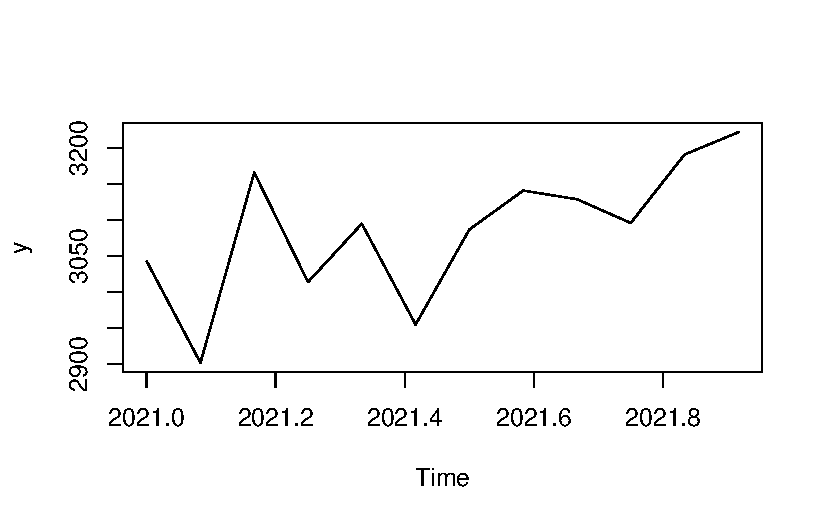
\includegraphics{intro_files/figure-pdf/unnamed-chunk-2-1.pdf}

Outros detalhes gráficos da função \texttt{plot} podem ser utilizados.

\begin{Shaded}
\begin{Highlighting}[]
\FunctionTok{plot}\NormalTok{(y, }\AttributeTok{ylab =} \StringTok{\textquotesingle{}No. nascidos vivos\textquotesingle{}}\NormalTok{, }\AttributeTok{lwd =} \DecValTok{2}\NormalTok{, }\AttributeTok{col =} \StringTok{\textquotesingle{}seagreen\textquotesingle{}}\NormalTok{, }\AttributeTok{xlab =} \StringTok{\textquotesingle{}Ano\textquotesingle{}}\NormalTok{, }\AttributeTok{main =} \StringTok{\textquotesingle{}Série mensal de nascidos vivos em Manaus\textquotesingle{}}\NormalTok{, }\AttributeTok{sub=}\StringTok{\textquotesingle{}Fonte: Sistema de Informação sobre Nascidos Vivos/SUS\textquotesingle{}}\NormalTok{)}
\end{Highlighting}
\end{Shaded}

\includegraphics{intro_files/figure-pdf/unnamed-chunk-3-1.pdf}

É possível extrair os argumentos de um \texttt{ts} já criado utilizando
funções com os mesmos nomes dos respectivos argumentos. No exemplo
acima, criamos o objeto denominado \texttt{y}. Abaixo, extraímos os
argumentos deste objeto.

\begin{Shaded}
\begin{Highlighting}[]
\FunctionTok{start}\NormalTok{(y)}
\end{Highlighting}
\end{Shaded}

\begin{verbatim}
[1] 2021    1
\end{verbatim}

\begin{Shaded}
\begin{Highlighting}[]
\FunctionTok{end}\NormalTok{(y)}
\end{Highlighting}
\end{Shaded}

\begin{verbatim}
[1] 2021   12
\end{verbatim}

\begin{Shaded}
\begin{Highlighting}[]
\FunctionTok{frequency}\NormalTok{(y)}
\end{Highlighting}
\end{Shaded}

\begin{verbatim}
[1] 12
\end{verbatim}

\begin{Shaded}
\begin{Highlighting}[]
\FunctionTok{deltat}\NormalTok{(y)}
\end{Highlighting}
\end{Shaded}

\begin{verbatim}
[1] 0.08333333
\end{verbatim}

A função \texttt{window} é particularmente útil para selecionar um
subconjunto da série temporal. Seus argumentos são os mesmos da função
\texttt{ts}.

\textbf{Exemplo} Utilizando o mesmo conjunto de dados do exemplo
anterior, vamos usar a função \texttt{window} para extrair apenas os
nascimentos entre junho e agosto.

\begin{Shaded}
\begin{Highlighting}[]
\NormalTok{z }\OtherTok{\textless{}{-}} \FunctionTok{window}\NormalTok{(y, }\AttributeTok{start=}\FunctionTok{c}\NormalTok{(}\DecValTok{2021}\NormalTok{,}\DecValTok{6}\NormalTok{), }\AttributeTok{end =} \FunctionTok{c}\NormalTok{(}\DecValTok{2021}\NormalTok{,}\DecValTok{8}\NormalTok{))}
\NormalTok{z}
\end{Highlighting}
\end{Shaded}

\begin{verbatim}
      Jun  Jul  Aug
2021 2955 3087 3141
\end{verbatim}

Acima, \texttt{z} é um novo objeto \texttt{ts}. Podemos usar a função
\texttt{lines} destacar a parte selecionada da série em um gráfico já
existente. Abaixo, descatamos os dados selecionados em \texttt{z}.

\begin{Shaded}
\begin{Highlighting}[]
\FunctionTok{plot}\NormalTok{(y, }\AttributeTok{ylab =} \StringTok{\textquotesingle{}No. nascidos vivos\textquotesingle{}}\NormalTok{, }\AttributeTok{lwd =} \DecValTok{2}\NormalTok{, }\AttributeTok{col =} \StringTok{\textquotesingle{}seagreen\textquotesingle{}}\NormalTok{, }\AttributeTok{xlab =} \StringTok{\textquotesingle{}Ano\textquotesingle{}}\NormalTok{, }\AttributeTok{main =} \StringTok{\textquotesingle{}Série }
\StringTok{mensal de nascidos vivos em Manaus\textquotesingle{}}\NormalTok{, }\AttributeTok{sub=}\StringTok{\textquotesingle{}Fonte: Sistema de Informação sobre Nascidos Vivos/SUS\textquotesingle{}}\NormalTok{)}
\FunctionTok{lines}\NormalTok{(z, }\AttributeTok{col =}\StringTok{\textquotesingle{}brown\textquotesingle{}}\NormalTok{, }\AttributeTok{lwd =} \DecValTok{4}\NormalTok{ )}
\end{Highlighting}
\end{Shaded}

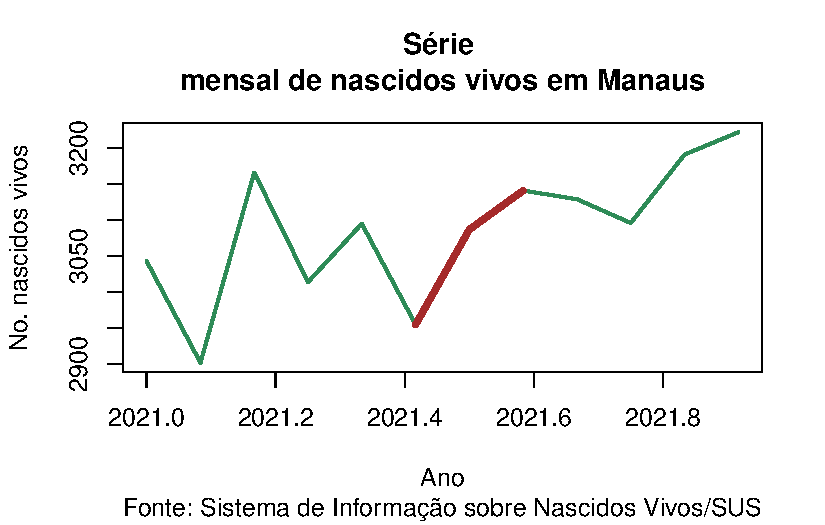
\includegraphics{intro_files/figure-pdf/unnamed-chunk-6-1.pdf}

Exercício 1

A série abaixo representa o número de homicídios mensais no Amazonas,
segundo causa básica de óbito, entre os anos 2000 e 2023.

\begin{Shaded}
\begin{Highlighting}[]
\FunctionTok{require}\NormalTok{(gsheet)}
\NormalTok{url }\OtherTok{=} \StringTok{\textquotesingle{}https://docs.google.com/spreadsheets/d/1rtiyOZ1W3SRIWZJTR1RyBmxmnGO11x005GNGrgLBr5A/edit?usp=sharing\textquotesingle{}}

\NormalTok{hom }\OtherTok{=} \FunctionTok{gsheet2tbl}\NormalTok{(url)}
\end{Highlighting}
\end{Shaded}

\begin{enumerate}
\def\labelenumi{\arabic{enumi}.}
\item
  Construa um objeto do tipo \texttt{ts}
\item
  Faça um gráfico da série.
\item
  Crie um janela para marcar o período entre o início da pandemia de
  COVID-19 (março de 2020) e o primeiro dia sem mortes por COVID-19
  (julho de 2021)
\item
  Represente a janela acima no gráfico anterior. O que esse gráfico
  revela?
\end{enumerate}

\section{\texorpdfstring{A classe \texttt{Date} e o pacote
\texttt{lubridate}}{A classe Date e o pacote lubridate}}\label{a-classe-date-e-o-pacote-lubridate}

Nessa seção discutimos a classe \texttt{Date}, responsável por operações
com datas no \texttt{R}. São apresentadas as principais funções do
pacote \texttt{base}. Em seguida, apresentamos o pacote
\texttt{lubridate}, que oferece funções adicionais e uma sintaxe mais
fluida.

No pacote \texttt{base}, as datas são objeto da classe \texttt{Date}.
Abaixo, transformamos o texto que representa 3 de agosto de 1998 nessa
classe.

\begin{Shaded}
\begin{Highlighting}[]
\CommentTok{\# 3 de agosto de 1998 (formato americano)}
\NormalTok{x }\OtherTok{\textless{}{-}} \StringTok{\textquotesingle{}1998/8/3\textquotesingle{}}
\NormalTok{y }\OtherTok{\textless{}{-}} \FunctionTok{as.Date}\NormalTok{(x)}
\end{Highlighting}
\end{Shaded}

Existem diversas funções que interagem com objetos nessa classe:

\begin{itemize}
\item
  \texttt{weekdays}: Retorna o dia da semana.
\item
  \texttt{months}: Retorna o nome do mês.
\item
  \texttt{quarters}: Retorna o trimestre do ano (Q1,Q2,Q3 ou Q4).
\end{itemize}

Abaixo, ilustramos o uso dessas funções com a data 3 de agosto de 1998.

\begin{Shaded}
\begin{Highlighting}[]
\FunctionTok{weekdays}\NormalTok{(y)}
\end{Highlighting}
\end{Shaded}

\begin{verbatim}
[1] "segunda-feira"
\end{verbatim}

\begin{Shaded}
\begin{Highlighting}[]
\FunctionTok{months}\NormalTok{(y)}
\end{Highlighting}
\end{Shaded}

\begin{verbatim}
[1] "agosto"
\end{verbatim}

\begin{Shaded}
\begin{Highlighting}[]
\FunctionTok{quarters}\NormalTok{(y)}
\end{Highlighting}
\end{Shaded}

\begin{verbatim}
[1] "Q3"
\end{verbatim}

Outra vantagem desta classe é a possibilidade de calcular a diferença em
dias entre duas datas, utilizando a função \texttt{-}. Abaixo mostramos
a diferença entre 3 de agosto de 1998 e 3 de agosto de 1999.

\begin{Shaded}
\begin{Highlighting}[]
\NormalTok{z }\OtherTok{\textless{}{-}} \FunctionTok{as.Date}\NormalTok{(}\StringTok{\textquotesingle{}1999{-}08{-}03\textquotesingle{}}\NormalTok{)}
\NormalTok{z}\SpecialCharTok{{-}}\NormalTok{y}
\end{Highlighting}
\end{Shaded}

\begin{verbatim}
Time difference of 365 days
\end{verbatim}

Em certas aplicações, é necessário criar um vetor contendo datas em
sequência. A função \texttt{seq} interage com objetos da classe
\texttt{Date}, permitindo que o argumento \texttt{by} receba as strings
\texttt{day}, \texttt{week},\texttt{month}, \texttt{quarter} e
\texttt{year}. Abaixo, criamos um vetor mensal que começa em 3 de agosto
de 1998 e terminando e 3 de agosto de 1999.

\begin{Shaded}
\begin{Highlighting}[]
\NormalTok{inicio }\OtherTok{\textless{}{-}} \FunctionTok{as.Date}\NormalTok{(}\StringTok{\textquotesingle{}1998{-}08{-}03\textquotesingle{}}\NormalTok{)}
\NormalTok{fim }\OtherTok{\textless{}{-}} \FunctionTok{as.Date}\NormalTok{(}\StringTok{\textquotesingle{}1999{-}08{-}03\textquotesingle{}}\NormalTok{)}
\FunctionTok{seq}\NormalTok{(inicio, fim, }\AttributeTok{by=}\StringTok{\textquotesingle{}month\textquotesingle{}}\NormalTok{)}
\end{Highlighting}
\end{Shaded}

\begin{verbatim}
 [1] "1998-08-03" "1998-09-03" "1998-10-03" "1998-11-03" "1998-12-03"
 [6] "1999-01-03" "1999-02-03" "1999-03-03" "1999-04-03" "1999-05-03"
[11] "1999-06-03" "1999-07-03" "1999-08-03"
\end{verbatim}

Observe que a conversão da \texttt{string} para \texttt{Date} é
realizada considerando o formato americano por padrão. É possível usar a
função \texttt{as.Date} para ler qualquer formato, modificando o
argumento \texttt{format}. No entanto, o pacote \texttt{lubridate}
oferece funções mais simples para essa conversão:

\begin{itemize}
\item
  \texttt{ymd}: Converte \texttt{strings} no formato ``ano, mês, dia'',
  como ``2023-10-26''.
\item
  \texttt{mdy}: Converte \texttt{strings} no formato ``mês, dia, ano'',
  como ``10-26-2023''.
\item
  \texttt{dmy}: Converte \texttt{strings} no formato ``dia, mês, ano'',
  como ``26-10-2023''.
\end{itemize}

Abaixo, transformamos a data 3/8/1998 para o formato americano.

\begin{Shaded}
\begin{Highlighting}[]
\FunctionTok{require}\NormalTok{(lubridate)}
\CommentTok{\# 3 de agosto de 1998 (formato nacional)}
\NormalTok{x }\OtherTok{\textless{}{-}} \StringTok{\textquotesingle{}3/8/1998\textquotesingle{}}
\FunctionTok{dmy}\NormalTok{(x)}
\end{Highlighting}
\end{Shaded}

\begin{verbatim}
[1] "1998-08-03"
\end{verbatim}

O \texttt{lubridate} também ofere a possibilidade de trabalhar com
informações de tempo dentro de um dia, como horas, minutos e segundos.
Por exemplo, a informação 15h30 de 3 de agosto de 1998 é lida como

\begin{Shaded}
\begin{Highlighting}[]
\NormalTok{x }\OtherTok{\textless{}{-}} \StringTok{\textquotesingle{}3/8/1998 15:30:00\textquotesingle{}}
\FunctionTok{dmy\_hms}\NormalTok{(x)}
\end{Highlighting}
\end{Shaded}

\begin{verbatim}
[1] "1998-08-03 15:30:00 UTC"
\end{verbatim}

O \texttt{lubridate} possui as funções \texttt{month} e \texttt{wday},
que funcionam de modo análgo às funções \texttt{months} e
\texttt{weekdays}. Além disso, o \texttt{lubridate} traz uma série de
funções adicionais como:

\begin{itemize}
\tightlist
\item
  \texttt{year}: retorna o ano de uma data
\item
  \texttt{day}: retornam o dia de uma data (útil para o formado
  xxx-xx-xx 00:00:00)
\item
  \texttt{hour}, \texttt{minute}, \texttt{second}: Retornam a hora,
  minuto e segundo de um objeto de data e tempo.
\end{itemize}

As funções de arredondamento de data também são úteis, especialmente
para obter contagens mensais, anuais, etc. Elas são \texttt{floor\_date}
e \texttt{ceiling\_date} e são responsáveis por arredondar uma data para
o início ou o fim de um período, respectivamente. Abaixo, arredondamos a
data 3 de agosto de 1998 para o começo do mês.

\begin{Shaded}
\begin{Highlighting}[]
\NormalTok{x }\OtherTok{\textless{}{-}} \FunctionTok{dmy}\NormalTok{(}\StringTok{\textquotesingle{}03/08/1998\textquotesingle{}}\NormalTok{)}
\FunctionTok{floor\_date}\NormalTok{(x, }\StringTok{\textquotesingle{}month\textquotesingle{}}\NormalTok{)}
\end{Highlighting}
\end{Shaded}

\begin{verbatim}
[1] "1998-08-01"
\end{verbatim}

\textbf{Exemplo}

A Força Aérea Brasileira (FAB), por meio do Centro de Investigação e
Prevenção de Acidentes Aeronáuticos (CENIPA), possui um
\texttt{dashboard} para explorar dados sobre incidentes e acidentes
aéreos no Brasil. Um acidente é definido como uma ocorrência grave
associada à operação de uma aeronave que resulta em lesões ou morte,
dano estrutural da aeronave ou aeronave desaparecida. Os demais casos
são classificados como incidentes. Os dados, atualizados em 11/08/2025,
estão disponíveis para esse curso na \texttt{url} abaixo:

\begin{Shaded}
\begin{Highlighting}[]
\NormalTok{url }\OtherTok{\textless{}{-}} \StringTok{\textquotesingle{}https://docs.google.com/spreadsheets/d/1BjTXFMmTpcxKdRHCr5IIDJde9yr0s3oAAfyj2vdVuX8/edit?usp=sharing\textquotesingle{}}

\NormalTok{aereo }\OtherTok{\textless{}{-}}  \FunctionTok{gsheet2tbl}\NormalTok{(url)}
\FunctionTok{head}\NormalTok{(aereo)}
\end{Highlighting}
\end{Shaded}

\begin{verbatim}
# A tibble: 6 x 10
  Link   Data  Matrícula Classificação Tipo  Localidade UF    Aeródromo Operação
  <chr>  <chr> <chr>     <chr>         <chr> <chr>      <chr> <chr>     <chr>   
1 https~ 05/0~ ****      INCIDENTE     FALH~ RIO DE JA~ RJ    FAER      TÁXI AÉ~
2 https~ 04/0~ ****      INCIDENTE     FALH~ MARICÁ     RJ    NCAD      TÁXI AÉ~
3 https~ 01/0~ ****      INCIDENTE     FALH~ RIO DE JA~ RJ    SBJR      TÁXI AÉ~
4 https~ 31/0~ ****      INCIDENTE     FALH~ PALMAS     TO    SBPJ      REGULAR 
5 https~ 29/0~ ****      INCIDENTE     FALH~ BOA VISTA  RR    FAER      TÁXI AÉ~
6 https~ 29/0~ ****      INCIDENTE     COLI~ RECIFE     PE    SBRF      REGULAR 
# i 1 more variable: Status <chr>
\end{verbatim}

A unidade amostral é o acidente/indicente. Estamos interessados em criar
uma série temporal com o número de acidentes mensais. Abaixo, filtramos
apenas os acidentes (coluna \texttt{Classificção}) e, em seguida,
transformamos as datas em objetos do tipo \texttt{Date}.

\begin{Shaded}
\begin{Highlighting}[]
\NormalTok{acidentes }\OtherTok{\textless{}{-}}\NormalTok{ aereo[ aereo}\SpecialCharTok{$}\NormalTok{Classificação}\SpecialCharTok{==}\StringTok{\textquotesingle{}ACIDENTE\textquotesingle{}}\NormalTok{, ]}
\NormalTok{datas }\OtherTok{\textless{}{-}} \FunctionTok{dmy}\NormalTok{(acidentes}\SpecialCharTok{$}\NormalTok{Data)}
\end{Highlighting}
\end{Shaded}

Agora, vamos arredondar todas as datas para o primeiro dia do mês. Em
seguida, contaremos as frequências para cada mês/ano

\begin{Shaded}
\begin{Highlighting}[]
\NormalTok{mes\_ano }\OtherTok{\textless{}{-}} \FunctionTok{floor\_date}\NormalTok{(datas, }\StringTok{\textquotesingle{}month\textquotesingle{}}\NormalTok{)}
\NormalTok{contagem }\OtherTok{\textless{}{-}} \FunctionTok{table}\NormalTok{(mes\_ano)}
\NormalTok{contagem}
\end{Highlighting}
\end{Shaded}

\begin{verbatim}
mes_ano
2015-01-01 2015-02-01 2015-03-01 2015-04-01 2015-05-01 2015-06-01 2015-07-01 
        12         14         15         19         16         14         16 
2015-08-01 2015-09-01 2015-10-01 2015-11-01 2015-12-01 2016-01-01 2016-02-01 
        13         17          9         14         13         20         16 
2016-03-01 2016-04-01 2016-05-01 2016-06-01 2016-07-01 2016-08-01 2016-09-01 
        20         19          8          5         11          4         17 
2016-10-01 2016-11-01 2016-12-01 2017-01-01 2017-02-01 2017-03-01 2017-04-01 
        20          9         15         17         16         11         16 
2017-05-01 2017-06-01 2017-07-01 2017-08-01 2017-09-01 2017-10-01 2017-11-01 
         8          6         12          6         14         15         16 
2017-12-01 2018-01-01 2018-02-01 2018-03-01 2018-04-01 2018-05-01 2018-06-01 
         9         18         19         18         18         15         13 
2018-07-01 2018-08-01 2018-09-01 2018-10-01 2018-11-01 2018-12-01 2019-01-01 
        15          8         11          8         14         10         20 
2019-02-01 2019-03-01 2019-04-01 2019-05-01 2019-06-01 2019-07-01 2019-08-01 
        10         17         14         12         13         15          8 
2019-09-01 2019-10-01 2019-11-01 2019-12-01 2020-01-01 2020-02-01 2020-03-01 
        14          6         11         11         11         17         12 
2020-04-01 2020-05-01 2020-06-01 2020-07-01 2020-08-01 2020-09-01 2020-10-01 
        14          9          6         16          9         15         18 
2020-11-01 2020-12-01 2021-01-01 2021-02-01 2021-03-01 2021-04-01 2021-05-01 
         7         16         13         16         17          7         17 
2021-06-01 2021-07-01 2021-08-01 2021-09-01 2021-10-01 2021-11-01 2021-12-01 
         5          8          8         12          7         13         18 
2022-01-01 2022-02-01 2022-03-01 2022-04-01 2022-05-01 2022-06-01 2022-07-01 
        15         12         13         13          9         13          8 
2022-08-01 2022-09-01 2022-10-01 2022-11-01 2022-12-01 2023-01-01 2023-02-01 
         8         12         10         13         12         21         21 
2023-03-01 2023-04-01 2023-05-01 2023-06-01 2023-07-01 2023-08-01 2023-09-01 
        18         12         17         15          7          6          5 
2023-10-01 2023-11-01 2023-12-01 2024-01-01 2024-02-01 2024-03-01 2024-04-01 
         8         14         11         17         21         12         22 
2024-05-01 2024-06-01 2024-07-01 2024-08-01 2024-09-01 2024-10-01 2024-11-01 
         7         15         13          9         13         12         14 
2024-12-01 2025-01-01 2025-02-01 2025-03-01 2025-04-01 2025-05-01 2025-06-01 
        20         22         11         13         20         10          5 
2025-07-01 
        11 
\end{verbatim}

É sempre importante checar o resultado em \texttt{contagem}, para
verificar se não há algum mês ausente. Como não o caso aqui, vamos
construir um objeto do tipo \texttt{ts} e fazer o gráfico da série
temporal.

\begin{Shaded}
\begin{Highlighting}[]
\NormalTok{serie }\OtherTok{\textless{}{-}} \FunctionTok{ts}\NormalTok{(contagem, }\AttributeTok{start=}\FunctionTok{c}\NormalTok{(}\DecValTok{2015}\NormalTok{,}\DecValTok{1}\NormalTok{), }\AttributeTok{frequency =} \DecValTok{12}\NormalTok{ )}
\FunctionTok{plot}\NormalTok{(serie, }\AttributeTok{ylab =} \StringTok{\textquotesingle{}No. de acidentes aéreos\textquotesingle{}}\NormalTok{, }\AttributeTok{xlab =} \StringTok{\textquotesingle{}Ano\textquotesingle{}}\NormalTok{, }\AttributeTok{sub=} \StringTok{\textquotesingle{}Fonte: CENIPA\textquotesingle{}}\NormalTok{ )}
\end{Highlighting}
\end{Shaded}

\includegraphics{intro_files/figure-pdf/unnamed-chunk-18-1.pdf}

Exercício 2

A série abaixo contém as datas dos óbitos maternos no Brasil a partir de
2010.

\begin{Shaded}
\begin{Highlighting}[]
\NormalTok{url }\OtherTok{\textless{}{-}} \StringTok{\textquotesingle{}https://drive.google.com/uc?authuser=0\&id=1tYFFT9L2iopKmBDUI3P8qNIRaOnMYj7d\&export=download\textquotesingle{}}
\end{Highlighting}
\end{Shaded}

Crie uma série temporal com o número de óbitos mensal e faça um gráfico.
Crie uma janela para destacar no gráfico o período da pandemia de
COVID-19 (março de 2020 até julhode 2021).

\bookmarksetup{startatroot}

\chapter{Sinal, ruído e
correlograma}\label{sinal-ruuxeddo-e-correlograma}

\section{Sinal e ruído}\label{sinal-e-ruuxeddo}

Em geral, a série temporal possui componentes de dois tipos: sinal e
ruído. O primeiro é uma função do tempo geralmente relacionado com a
média da série em dado instante de tempo, enquanto que o segundo está
relacionado com a variância. Podemos assumir que essa relação é aditiva:

\[X_t=\hbox{sinal}(t)+\varepsilon_t\] onde \(\varepsilon_t\) é o ruído.

Em alguns casos essa relação é multiplicativa, ou seja,

\[X_t=\exp\{\hbox{sinal}(t)+\varepsilon_t\},\] e, nesses casos,
aplicamos o logaritmo na série para que as componentes se tornem
aditivas.

Os sinais mais importantes são:

\begin{itemize}
\item
  Tendência: um comportamento de subida ou descida que pode ser
  observado no médio/longo prazo. Uma série temporal com tendência
  costuma ser bem representada por polinômios, ou seja
  \[x_t= \sum_{j=0}^q\beta_j t^j +\varepsilon_t.\]
\item
  Sazonalidade: é um padrão de oscilação que ocorre em um período fixo e
  conhecido. Cheias de rios e quantidade de chuva são exemplos de
  padrões sazonais. Em termos gerais, o padrão sazonal pode ser
  representado por um harmônico, ou seja,
\end{itemize}

\[x_t=A\cos\left(\phi+\frac{2\pi}{p}t\right)+\varepsilon_t\] onde \(p\)
é o período sazonal, \(A\) é amplitude da onda e \(\phi\) a fase.

\begin{itemize}
\tightlist
\item
  Ciclos: é um padrão oscilatório sem período fixo, como o ciclo de
  recessão de uma economia. Modelar ciclos é um pouco mais complexo, mas
  veremos posteriormente que é possível escrever séries deste tipo como
  \[x_t=A_t\cos\left(\phi_t+2\pi\lambda t\right)+\varepsilon_t,\] onde a
  amplitude e a fase variam no tempo e o período \(1/\lambda\) é
  desconhecido.
\end{itemize}

Os padrões oscilatórios (sazonalidade e ciclos) descritos acima variam
em torno de zero. Caso seja necessário, um parâmetro \(\mu\) constante
pode ser adicionado para caracterizar uma oscilação em torno de uma
média.

É possível que uma série possua todos os sinais acima, sendo escrita
como

\[x_t=\sum_{j=0}^q \beta_j t^j+A\cos\left(\phi+2\pi\lambda t\right)+A_t\cos\left(\phi_t+2\pi\lambda t\right)+\varepsilon_t\]

O ruído é a parte aleatória da composição e possui média zero. Isso
implica que, para uma série com sinal \(f(t)\), teremos

\[E(x_t)=E(f(t))+E(\varepsilon_t)=f(t)\] e
\[Var(x_t)=Var(f(t)+\varepsilon_t)=Var(\varepsilon_t)\] Os ruídos mais
importantes são:

\begin{itemize}
\item
  Ruído branco: possuem variância constante e são não correlacionados,
  ou seja \(Cov(\varepsilon_t,\varepsilon_s)=0\) para todo \(t\neq s\).
\item
  Média móvel de ordem \(q\): sejam
  \(\ldots,\varepsilon_{-2},\varepsilon_{-1},\varepsilon_{0},\varepsilon_{1},\ldots\)
  ruídos brancos. O ruído de média móvel de ordem \(q\) é dado por
  \[\eta_t=\varepsilon_{t}+\sum_{j=1}^q \theta_j\varepsilon_{t-j}.\]
\end{itemize}

A série a seguir representa uma série mensal de concentração de
\(\hbox{CO}_2\) na atmosfera em Mauna Loa, expressa em partes por
milhão. Note o comportamento da tendência e da sazonalidade.

\begin{Shaded}
\begin{Highlighting}[]
\FunctionTok{plot}\NormalTok{(co2)}
\end{Highlighting}
\end{Shaded}

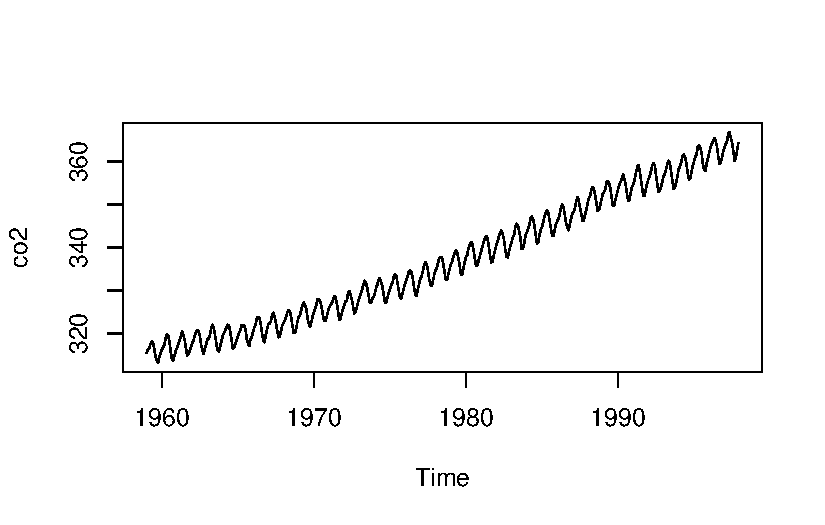
\includegraphics{sinal_files/figure-pdf/unnamed-chunk-1-1.pdf}

Existem diversas ferramentas que estimam a tendência e a sazonalidade.
Dentre estas, detaca-se o STL, por sua robustez. Abaixo, ilustramos a
decomposição da série \texttt{co2}. O termo \texttt{remainder}, também
conhecido como resíduo, é calculado como

\[e_t=x_t-\hat{f}(t),\] onde \(\hat{f}(t)\) é o sinal
(tendência+sazonalidade) ajustado. Se não houver qualquer outro sinal a
ser ajustado, então \(e_t\) é uma estimativa para \(\varepsilon_t\).

\begin{Shaded}
\begin{Highlighting}[]
\CommentTok{\# p é o período do padrão sazonal}
\NormalTok{p }\OtherTok{=} \DecValTok{12}
\FunctionTok{plot}\NormalTok{(}\FunctionTok{stl}\NormalTok{(co2,p))}
\end{Highlighting}
\end{Shaded}

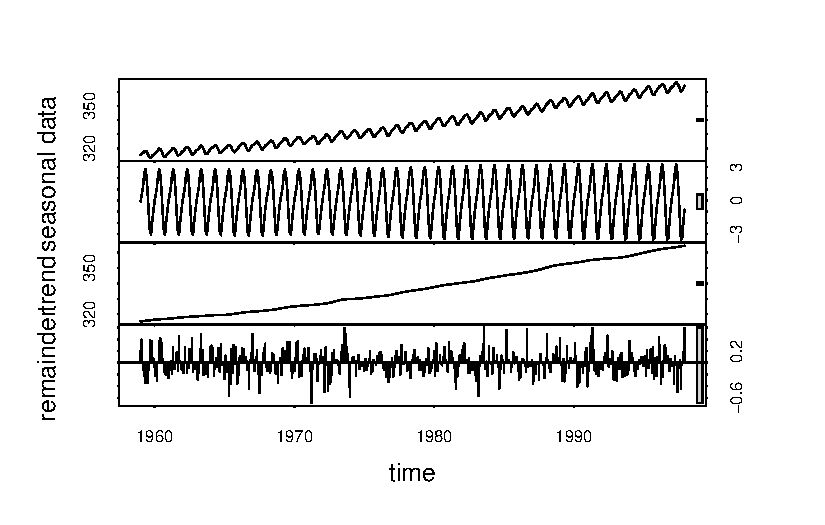
\includegraphics{sinal_files/figure-pdf/unnamed-chunk-2-1.pdf}

\textbf{Exercício.} Considere a série \texttt{AirPassengers}, disponível
no pacote \texttt{datasets}.

\begin{enumerate}
\def\labelenumi{\arabic{enumi}.}
\item
  Faça um gráfico da série temporal e procure determinar suas
  componentes.
\item
  A função \texttt{decompose} estima a sazonalidade assumindo a média
  das observações correspodentes ao mesmo fator sazonal (por exemplo,
  todos os janeiros). Faça um gráfico do resultado do \texttt{decompose}
  para esta série e discuta os resultados (em especial o termo
  \texttt{random}, que é o resíduo da decomposição).
\item
  Repita o item 2, mas utilizando a função \texttt{stl}. Quais são as
  principais diferenças?
\item
  Aplique o logaritmo da série e verifique o seu gráfico. Quais são as
  semelhanças e diferenças deste gráfico com o obtido no item 1?
\end{enumerate}

\textbf{Exercício.} Na série abaixo temos a taxa de desemprego mensal no
Brasil entre março de 2002 e dezembro de 2015. Analise as componentes
desta série.

\begin{Shaded}
\begin{Highlighting}[]
\NormalTok{url }\OtherTok{\textless{}{-}} \StringTok{\textquotesingle{}https://www.dropbox.com/s/rmgymzsic99qawd/desemprego.csv?dl=1\textquotesingle{}}
\NormalTok{banco }\OtherTok{\textless{}{-}} \FunctionTok{read.csv}\NormalTok{(url, }\AttributeTok{sep =} \StringTok{\textquotesingle{};\textquotesingle{}}\NormalTok{, }\AttributeTok{h =}\NormalTok{ F)}
\end{Highlighting}
\end{Shaded}

\section{A função de
aucorrelação}\label{a-funuxe7uxe3o-de-aucorrelauxe7uxe3o}

Considere inicialmente uma amostra aleatória \(X_1,\ldots,X_n\) (ou
seja, todas as variáveis são independentes e possuem a mesma
distribuição). Sejam \[A_h=\{X_1,\ldots,X_{n-h}\}\] e
\[B_h=\{X_h,\ldots,X_n\}.\] Então, a correlação entre \(A_h\) e \(B_h\)
é nula.

Deste modo, um meio de verificar se a coleção observada é uma série
temporal é observar a correlação amostral entre
\[a_h=\{x_1,\ldots,x_{n-h}\}\] e \[b_h=\{x_h,\ldots,x_n\},\] para
diferentes valores de \(h\).

A função \(r(h)\) que representa a correlação amostral entre \(a_h\) e
\(b_h\) é denominada \textbf{autocorrelação}. O valor \(h\) é denominado
\textbf{defasagem} (do inglês, \emph{lag}).

Propriedades

\begin{itemize}
\item
  \(r(0)=1\)
\item
  \(-1\leq r(h) \leq 1\)
\end{itemize}

Correlograma O gráfico \((h,r(h))\) é denominado correlograma, ou
gráfico da função de autocorrelação.

\subsection{O correlograma de uma amostra
aleatória}\label{o-correlograma-de-uma-amostra-aleatuxf3ria}

Quando a amostra é aleatória, a função de autocorrelação é nula para
qualquer defasagem diferente de 0. Deste modo, o correlograma deve
apresentar valores próximos de zero.

Para entender o que próximo de zero significa, o limites do intervalo de
confiança para o coeficiente de correlação sobre a hipótese de que esta
é nula são colocados no gráfico.

Abaixo ilustramos um correlograma para uma amostra de variáveis
aleatórias independentes com distribuição normal padrão.

\begin{Shaded}
\begin{Highlighting}[]
\NormalTok{x }\OtherTok{\textless{}{-}} \FunctionTok{rnorm}\NormalTok{(}\DecValTok{120}\NormalTok{)}

\CommentTok{\# correlograma}
\FunctionTok{acf}\NormalTok{(x)}
\end{Highlighting}
\end{Shaded}

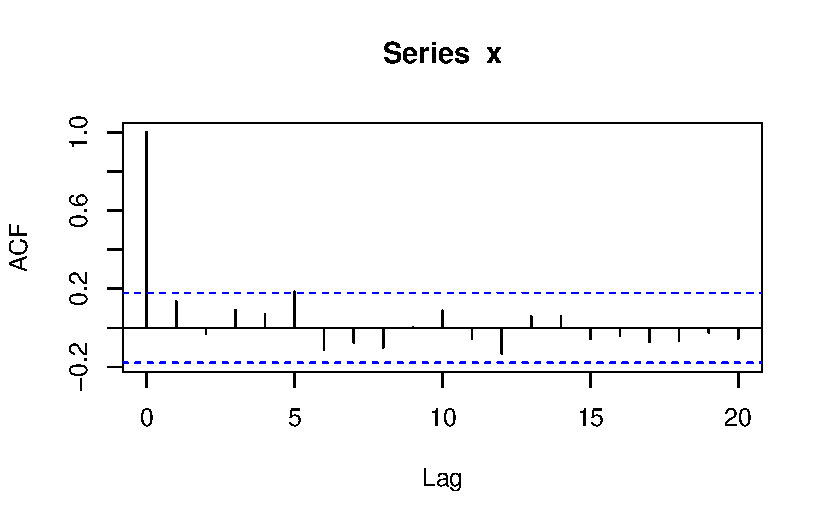
\includegraphics{sinal_files/figure-pdf/unnamed-chunk-4-1.pdf}

\begin{Shaded}
\begin{Highlighting}[]
\CommentTok{\# o mesmo correlograma com uma defasagem maior}
\FunctionTok{acf}\NormalTok{(x, }\AttributeTok{lag =} \DecValTok{50}\NormalTok{)}
\end{Highlighting}
\end{Shaded}

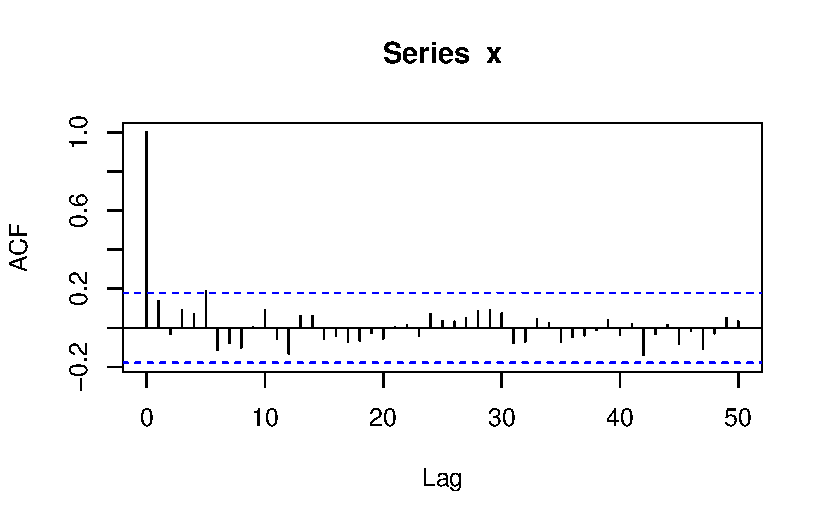
\includegraphics{sinal_files/figure-pdf/unnamed-chunk-4-2.pdf}

\subsection{O correlograma com a componente de
tendência}\label{o-correlograma-com-a-componente-de-tenduxeancia}

Quando uma série exibe tendência, o correlograma exibe um descaimento
lento e persistente.

Considere, por exemplo, a série

\[x_t= t + \varepsilon_t,\] onde
\(\varepsilon_t\sim\hbox{Normal}(0,5^2)\). Abaixo simulamos essa série e
apresentamos o respectivo correlograma

\begin{Shaded}
\begin{Highlighting}[]
\NormalTok{x }\OtherTok{\textless{}{-}} \FunctionTok{rnorm}\NormalTok{(}\DecValTok{100}\NormalTok{, }\DecValTok{1}\SpecialCharTok{:}\DecValTok{100}\NormalTok{, }\DecValTok{5}\NormalTok{)}

\NormalTok{oo }\OtherTok{\textless{}{-}} \FunctionTok{par}\NormalTok{( }\AttributeTok{mfrow=}\FunctionTok{c}\NormalTok{(}\DecValTok{1}\NormalTok{,}\DecValTok{2}\NormalTok{))}
\FunctionTok{ts.plot}\NormalTok{(x)}
\FunctionTok{acf}\NormalTok{(x, }\AttributeTok{lag =} \DecValTok{50}\NormalTok{)}
\end{Highlighting}
\end{Shaded}

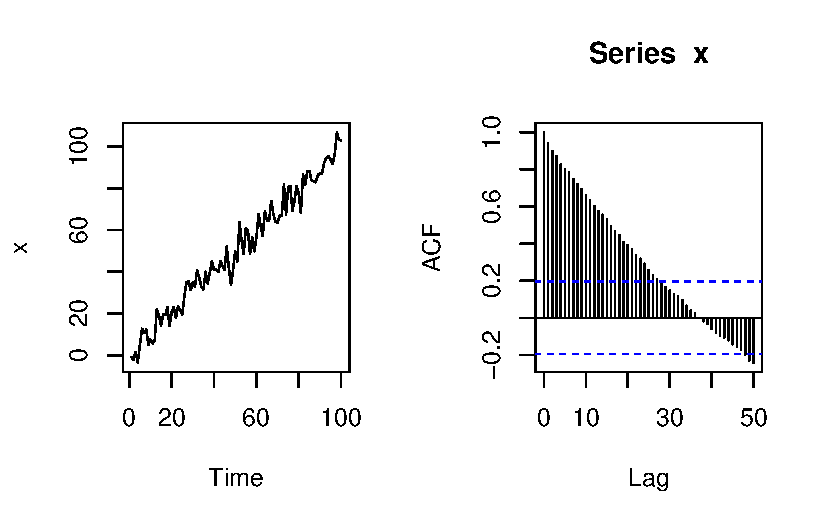
\includegraphics{sinal_files/figure-pdf/unnamed-chunk-5-1.pdf}

\begin{Shaded}
\begin{Highlighting}[]
\FunctionTok{par}\NormalTok{(oo)}
\end{Highlighting}
\end{Shaded}

Observe as similaridades do correlograma acima com o observado para a
série de acidentes aéreos mensais vista anteriormente.

\begin{Shaded}
\begin{Highlighting}[]
\NormalTok{oo }\OtherTok{\textless{}{-}} \FunctionTok{par}\NormalTok{( }\AttributeTok{mfrow=}\FunctionTok{c}\NormalTok{(}\DecValTok{1}\NormalTok{,}\DecValTok{2}\NormalTok{))}
\FunctionTok{ts.plot}\NormalTok{( fab\_mes , }\AttributeTok{ylab =} \StringTok{\textquotesingle{}No. acidentes aéreos mensal\textquotesingle{}}\NormalTok{ )}
\FunctionTok{acf}\NormalTok{(fab\_mes , }\AttributeTok{lag =} \DecValTok{50}\NormalTok{,  }\AttributeTok{main =}\StringTok{\textquotesingle{}correlograma\textquotesingle{}}\NormalTok{)}
\end{Highlighting}
\end{Shaded}

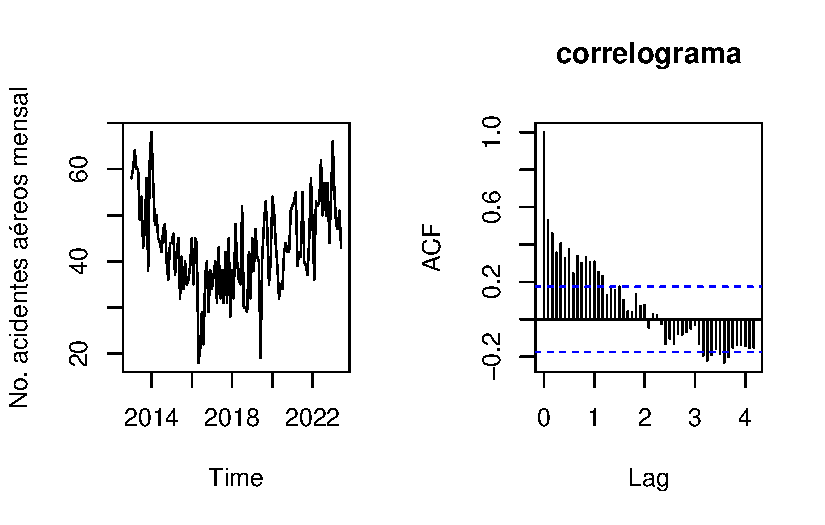
\includegraphics{sinal_files/figure-pdf/unnamed-chunk-7-1.pdf}

\begin{Shaded}
\begin{Highlighting}[]
\FunctionTok{par}\NormalTok{(oo)}
\end{Highlighting}
\end{Shaded}

\subsection{O correlograma com a componente de sazonalidade - sinal
harmônico}\label{o-correlograma-com-a-componente-de-sazonalidade---sinal-harmuxf4nico}

O sinal sazonal é caracterizado por um comportamento periódico. Existem
dois comportamentos sazonais típicos. O primeiro é baseado na função
harmônica:

\[\hbox{sinal}(t)=A\cos\left(\frac{2\pi}{p}t + \phi\right)\] Neste tipo
de sinal, há um comportamento em forma de onda já estabelecido. Eis
algumas informações importantes:

\begin{itemize}
\item
  O valor \(p\), denominado período, equivale ao tempo que demora para o
  padrão se repetir.
\item
  \(A\) é denominado amplitude e representa o maior/menor valor que este
  sinal pode aingir.
\item
  Por último, \(\phi\) é denominado fase, e serve basicamente para
  deslocar a onda.
\end{itemize}

Abaixo seguem alguns exemplos de harmônicos, todos com período 12:

\begin{Shaded}
\begin{Highlighting}[]
\NormalTok{oo }\OtherTok{\textless{}{-}} \FunctionTok{par}\NormalTok{( }\AttributeTok{cex =} \FloatTok{1.3}\NormalTok{)}
\FunctionTok{curve}\NormalTok{( }\FunctionTok{cos}\NormalTok{( x}\SpecialCharTok{*} \DecValTok{2}\SpecialCharTok{*}\NormalTok{pi}\SpecialCharTok{/}\DecValTok{12}\NormalTok{), }\DecValTok{0}\NormalTok{,}\DecValTok{24}\NormalTok{, }\AttributeTok{lwd =} \DecValTok{2}\NormalTok{, }\AttributeTok{ylab =} \FunctionTok{expression}\NormalTok{( }\FunctionTok{cos}\NormalTok{( }\DecValTok{2}\SpecialCharTok{*}\NormalTok{pi}\SpecialCharTok{*}\NormalTok{t}\SpecialCharTok{/}\DecValTok{12}\NormalTok{ )))}
\FunctionTok{abline}\NormalTok{(}\AttributeTok{h =} \DecValTok{0}\NormalTok{, }\AttributeTok{lty =} \DecValTok{2}\NormalTok{ )}
\FunctionTok{abline}\NormalTok{(}\AttributeTok{v=}\DecValTok{12}\NormalTok{, }\AttributeTok{lty =} \DecValTok{2}\NormalTok{)}
\end{Highlighting}
\end{Shaded}

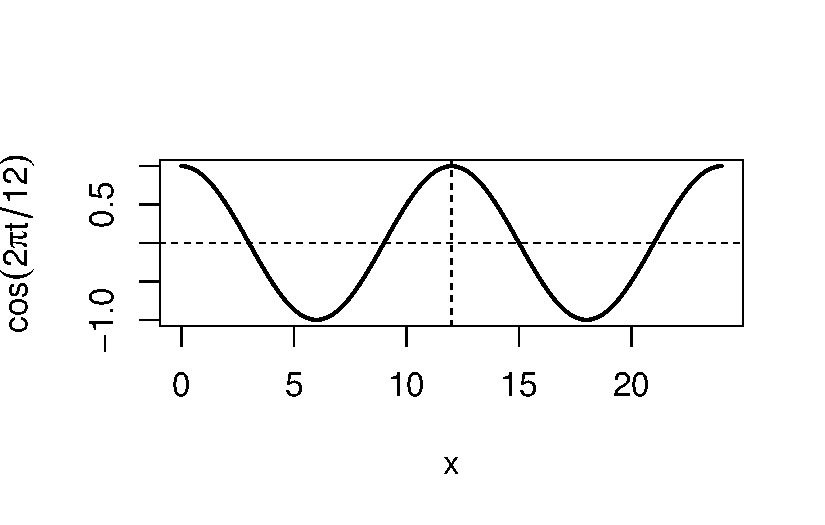
\includegraphics{sinal_files/figure-pdf/unnamed-chunk-8-1.pdf}

\begin{Shaded}
\begin{Highlighting}[]
\FunctionTok{curve}\NormalTok{( .}\DecValTok{5}\SpecialCharTok{*}\FunctionTok{cos}\NormalTok{( x}\SpecialCharTok{*} \DecValTok{2}\SpecialCharTok{*}\NormalTok{pi}\SpecialCharTok{/}\DecValTok{12}\NormalTok{), }\DecValTok{0}\NormalTok{,}\DecValTok{24}\NormalTok{, }\AttributeTok{lwd =} \DecValTok{2}\NormalTok{, }\AttributeTok{ylab =} \FunctionTok{expression}\NormalTok{( .}\DecValTok{5}\SpecialCharTok{*}\FunctionTok{cos}\NormalTok{( }\DecValTok{2}\SpecialCharTok{*}\NormalTok{pi}\SpecialCharTok{*}\NormalTok{t}\SpecialCharTok{/}\DecValTok{12}\NormalTok{ )), }\AttributeTok{ylim =} \FunctionTok{c}\NormalTok{(}\SpecialCharTok{{-}}\DecValTok{1}\NormalTok{,}\DecValTok{1}\NormalTok{))}
\FunctionTok{abline}\NormalTok{(}\AttributeTok{h =} \DecValTok{0}\NormalTok{, }\AttributeTok{lty =} \DecValTok{2}\NormalTok{ )}
\FunctionTok{abline}\NormalTok{(}\AttributeTok{v=}\DecValTok{12}\NormalTok{, }\AttributeTok{lty =} \DecValTok{2}\NormalTok{)}
\end{Highlighting}
\end{Shaded}

\includegraphics{sinal_files/figure-pdf/unnamed-chunk-8-2.pdf}

\begin{Shaded}
\begin{Highlighting}[]
\FunctionTok{curve}\NormalTok{( }\FunctionTok{cos}\NormalTok{( x}\SpecialCharTok{*} \DecValTok{2}\SpecialCharTok{*}\NormalTok{pi}\SpecialCharTok{/}\DecValTok{12}\SpecialCharTok{+}\DecValTok{90}\NormalTok{), }\DecValTok{0}\NormalTok{,}\DecValTok{24}\NormalTok{, }\AttributeTok{lwd =} \DecValTok{2}\NormalTok{, }\AttributeTok{ylab =} \FunctionTok{expression}\NormalTok{( }\FunctionTok{cos}\NormalTok{( }\DecValTok{2}\SpecialCharTok{*}\NormalTok{pi}\SpecialCharTok{*}\NormalTok{t}\SpecialCharTok{/}\DecValTok{12} \SpecialCharTok{+}\DecValTok{90}\NormalTok{)), }\AttributeTok{ylim =} \FunctionTok{c}\NormalTok{(}\SpecialCharTok{{-}}\DecValTok{1}\NormalTok{,}\DecValTok{1}\NormalTok{))}
\FunctionTok{abline}\NormalTok{(}\AttributeTok{h =} \DecValTok{0}\NormalTok{, }\AttributeTok{lty =} \DecValTok{2}\NormalTok{ )}
\FunctionTok{abline}\NormalTok{(}\AttributeTok{v=}\DecValTok{12}\NormalTok{, }\AttributeTok{lty =} \DecValTok{2}\NormalTok{)}
\end{Highlighting}
\end{Shaded}

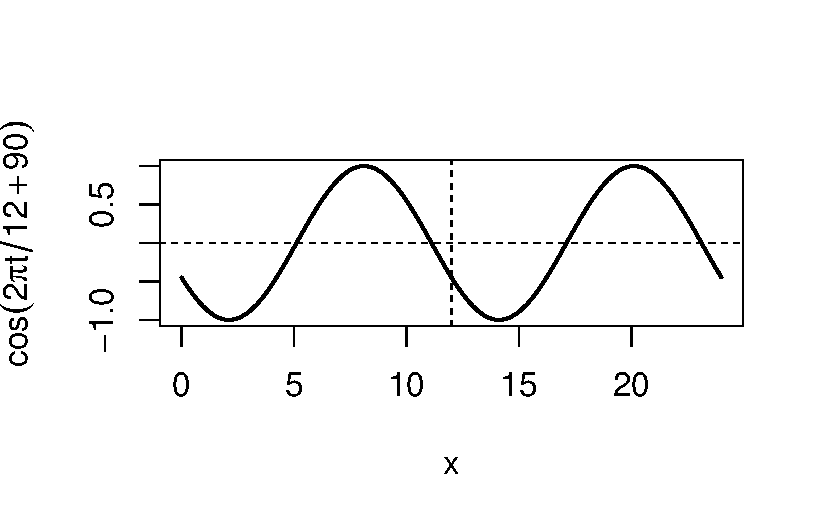
\includegraphics{sinal_files/figure-pdf/unnamed-chunk-8-3.pdf}

Abaixo simulamos uma série temporal com um sinal do tipo harmônico.
Observe que o comportamento em forma de onda é aparente na função de
autocorrelação.

\begin{Shaded}
\begin{Highlighting}[]
\NormalTok{x }\OtherTok{\textless{}{-}} \FunctionTok{cos}\NormalTok{( }\DecValTok{2}\SpecialCharTok{*}\NormalTok{pi}\SpecialCharTok{/}\DecValTok{12} \SpecialCharTok{*} \DecValTok{1}\SpecialCharTok{:}\DecValTok{100}\NormalTok{) }\SpecialCharTok{+} \FunctionTok{rnorm}\NormalTok{(}\DecValTok{100}\NormalTok{,}\DecValTok{0}\NormalTok{,.}\DecValTok{1}\NormalTok{)}

\NormalTok{oo }\OtherTok{\textless{}{-}} \FunctionTok{par}\NormalTok{( }\AttributeTok{mfrow =} \FunctionTok{c}\NormalTok{(}\DecValTok{1}\NormalTok{,}\DecValTok{2}\NormalTok{))}
\FunctionTok{ts.plot}\NormalTok{(x)}
\FunctionTok{acf}\NormalTok{(x)}
\end{Highlighting}
\end{Shaded}

\includegraphics{sinal_files/figure-pdf/unnamed-chunk-9-1.pdf}

\begin{Shaded}
\begin{Highlighting}[]
\FunctionTok{par}\NormalTok{(oo)}
\end{Highlighting}
\end{Shaded}

Abaixo, apresentamos a temperatura mensal observada no Castelo de
Nottingham, entre 1920-1939. Compare os resultados com os gráficos
acima.

\begin{Shaded}
\begin{Highlighting}[]
\NormalTok{oo }\OtherTok{\textless{}{-}} \FunctionTok{par}\NormalTok{( }\AttributeTok{mfrow =} \FunctionTok{c}\NormalTok{(}\DecValTok{1}\NormalTok{,}\DecValTok{2}\NormalTok{))}
  \FunctionTok{plot}\NormalTok{(nottem)}
  \FunctionTok{acf}\NormalTok{(nottem)}
\end{Highlighting}
\end{Shaded}

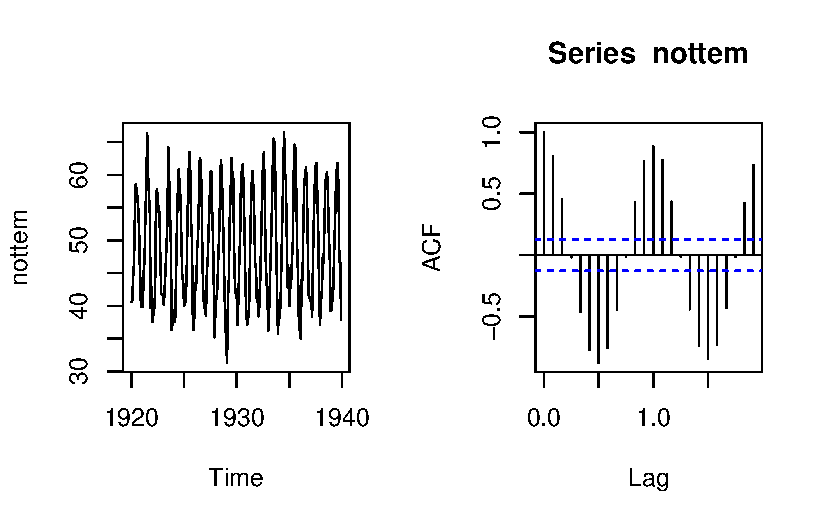
\includegraphics{sinal_files/figure-pdf/unnamed-chunk-10-1.pdf}

\begin{Shaded}
\begin{Highlighting}[]
\FunctionTok{par}\NormalTok{(oo)  }
\end{Highlighting}
\end{Shaded}

\subsection{O correlograma com a componente de sazonalidade - sinal
autorregressivo}\label{o-correlograma-com-a-componente-de-sazonalidade---sinal-autorregressivo}

Nesse tipo de sazonalidade, ainda há um período \(p\), mas não há um
sinal harmônico. O valor da série no tempo \(t\) é baseado no valor
observado no tempo \(t-p\).

Quando a sazonalidade possue essa característica, há uma autocorrelação
marcante nos múltiplos de \(p\). Observe a série simulada abaixo, com um
período \(p=12\)

\begin{Shaded}
\begin{Highlighting}[]
\FunctionTok{set.seed}\NormalTok{(}\DecValTok{123}\NormalTok{)}
\NormalTok{oo }\OtherTok{\textless{}{-}} \FunctionTok{par}\NormalTok{( }\AttributeTok{mfrow =} \FunctionTok{c}\NormalTok{(}\DecValTok{1}\NormalTok{,}\DecValTok{2}\NormalTok{))}
\NormalTok{x }\OtherTok{\textless{}{-}} \FunctionTok{rnorm}\NormalTok{(}\DecValTok{12}\NormalTok{,}\DecValTok{0}\NormalTok{,.}\DecValTok{1}\NormalTok{)}
\ControlFlowTok{for}\NormalTok{(i }\ControlFlowTok{in} \DecValTok{13}\SpecialCharTok{:}\DecValTok{100}\NormalTok{) x[i] }\OtherTok{\textless{}{-}}\NormalTok{ .}\DecValTok{6}\SpecialCharTok{*}\NormalTok{x[i}\DecValTok{{-}12}\NormalTok{] }\SpecialCharTok{+} \FunctionTok{rnorm}\NormalTok{(}\DecValTok{1}\NormalTok{,}\DecValTok{0}\NormalTok{,.}\DecValTok{05}\NormalTok{)}
\FunctionTok{ts.plot}\NormalTok{(x)}
\FunctionTok{acf}\NormalTok{(x, }\AttributeTok{lag =} \DecValTok{50}\NormalTok{)}
\end{Highlighting}
\end{Shaded}

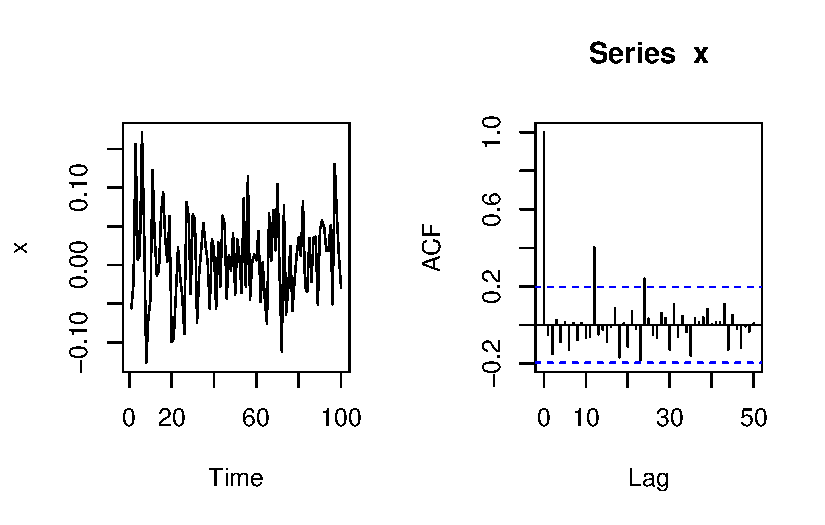
\includegraphics{sinal_files/figure-pdf/unnamed-chunk-11-1.pdf}

\begin{Shaded}
\begin{Highlighting}[]
\FunctionTok{par}\NormalTok{(oo)}
\end{Highlighting}
\end{Shaded}

\section{Exercícios}\label{exercuxedcios}

Exercício 1 Estude o comportamento da série \texttt{ldeaths}, que conta
o número mensal de óbitos por doenças pulmonares no Reino Unido.

Exercício 2 Estude o comportamento da série do número de óbitos maternos
mensais.

Exercício 3 Em 2017, um epidemiologista estava interessado na série de
suicídios no Mato Grosso do Sul. O banco de dados utilizado é dado a
seguir. Construa uma série mensal e estude seu comportamento

\begin{Shaded}
\begin{Highlighting}[]
\NormalTok{url }\OtherTok{\textless{}{-}} \StringTok{\textquotesingle{}https://drive.google.com/uc?authuser=0\&id=1DMSgrQDl0636Lw0Y0MYJHJrgw\_2uXntM\&export=download\textquotesingle{}}
\end{Highlighting}
\end{Shaded}

\bookmarksetup{startatroot}

\chapter{O modelo linear dinâmico}\label{o-modelo-linear-dinuxe2mico}

\section{O modelo linear dinâmico}\label{o-modelo-linear-dinuxe2mico-1}

Seja \(y_1,\ldots,t\) uma série temporal. Seja \(D_j={y_1,\ldots,y_j}\).
Dizemos que \(y_t\) é um modelo linear dinâmico se

\[\begin{align}
y_t|\boldsymbol{\theta}_t,D_{t-1}&\sim\hbox{Normal}(\boldsymbol{F}_t'\boldsymbol{\theta}_t,V_t)\\
\boldsymbol{\theta}_t|\boldsymbol{\theta}_{t-1},D_{t-1}&\sim\hbox{Normal}(\boldsymbol{G}_t\boldsymbol{\theta}_{t-1},\boldsymbol{W}_t)
\end{align}\]

A expressão acima, os \(\theta\)'s são denominados estados. Para a
completa especificação do modelo, devemos informar valores iniciais
\(m_0\) e \(C_0\) que representam nossa opinião sobre os estados antes
do tempo \(1\):

\[\theta_0\sim\ N(m_0,C_0)\] Escolhas diferentes para
\(\boldsymbol{F}_t\) e \(\boldsymbol{G}_t\) permitem acomodar sinais
diferentes.

Pode-se mostrar que \(y_{t+h}|D_t\) tem distribuição normal. Como
\(t+h\) é um tempo não observado, essa é a distribuição para previsões.
Neste caso, a função de previsão para o horizonte \(h\) é

\[f_t(h)=E(Y_{t+h}|D_{t})\] onde \(E(.)\) sempre deve ser lido como
\textbf{média}.

O pacote para lidar com modelos lineares dinâmicos é o \texttt{dlm}. A
função abaixo é utilizada para estimar as variâncias desconhecidas do
modelo e deve sempre ser colocada no \emph{environment} do \texttt{R}:

\begin{Shaded}
\begin{Highlighting}[]
\FunctionTok{require}\NormalTok{(dlm)}
\end{Highlighting}
\end{Shaded}

\begin{verbatim}
Carregando pacotes exigidos: dlm
\end{verbatim}

\begin{Shaded}
\begin{Highlighting}[]
\NormalTok{modFim }\OtherTok{\textless{}{-}} \ControlFlowTok{function}\NormalTok{(y,mod)\{}
\NormalTok{  ffbs }\OtherTok{\textless{}{-}} \FunctionTok{dlmGibbsDIG}\NormalTok{(y, }\AttributeTok{mod =}\NormalTok{ mod, }\AttributeTok{n.sample =} \DecValTok{5000}\NormalTok{,}
                    \AttributeTok{a.y=}\DecValTok{1}\NormalTok{,}\AttributeTok{b.y=}\DecValTok{100}\NormalTok{,}\AttributeTok{a.theta=}\DecValTok{1}\NormalTok{,}\AttributeTok{b.theta=}\DecValTok{100}\NormalTok{,}
                    \AttributeTok{save.states =} \ConstantTok{FALSE}\NormalTok{, }\AttributeTok{thin =} \DecValTok{0}\NormalTok{)}

\NormalTok{v\_sim  }\OtherTok{\textless{}{-}} \FunctionTok{sample}\NormalTok{(ffbs}\SpecialCharTok{$}\NormalTok{dV[}\SpecialCharTok{{-}}\NormalTok{(}\DecValTok{1}\SpecialCharTok{:}\DecValTok{2500}\NormalTok{)],}\DecValTok{2500}\NormalTok{,T)}

\NormalTok{q }\OtherTok{\textless{}{-}} \FunctionTok{dim}\NormalTok{(ffbs}\SpecialCharTok{$}\NormalTok{dW)[}\DecValTok{2}\NormalTok{]}
\NormalTok{w\_sim }\OtherTok{\textless{}{-}} \ConstantTok{NULL}
\ControlFlowTok{for}\NormalTok{(j }\ControlFlowTok{in} \DecValTok{1}\SpecialCharTok{:}\NormalTok{q)\{}
\NormalTok{ w\_sim }\OtherTok{\textless{}{-}} \FunctionTok{c}\NormalTok{(w\_sim, }\FunctionTok{mean}\NormalTok{(}\FunctionTok{sample}\NormalTok{(ffbs}\SpecialCharTok{$}\NormalTok{dW[,j][}\SpecialCharTok{{-}}\NormalTok{(}\DecValTok{1}\SpecialCharTok{:}\DecValTok{2500}\NormalTok{)],}\DecValTok{2500}\NormalTok{,T)))}
\NormalTok{\}}
\CommentTok{\# declarando as variâncias na quádrupla}
\NormalTok{mod}\SpecialCharTok{$}\NormalTok{V }\OtherTok{\textless{}{-}} \FunctionTok{mean}\NormalTok{(v\_sim)}
\NormalTok{mod}\SpecialCharTok{$}\NormalTok{W }\OtherTok{\textless{}{-}} \FunctionTok{diag}\NormalTok{( w\_sim)}
\FunctionTok{return}\NormalTok{(mod)}
\NormalTok{\}}
\end{Highlighting}
\end{Shaded}

Também pode-se mostrar que \(\theta_{t-h}|D_t\) tem distribuição normal.
Como se trata da distribuição dos estados após verificar toda a série
temporal, esta é a distribuição para a suavização.

\bookmarksetup{startatroot}

\chapter{Modelo linear dinâmico
polinomial}\label{modelo-linear-dinuxe2mico-polinomial}

\begin{Shaded}
\begin{Highlighting}[]
\FunctionTok{require}\NormalTok{(dlm)}
\end{Highlighting}
\end{Shaded}

\begin{verbatim}
Carregando pacotes exigidos: dlm
\end{verbatim}

\begin{Shaded}
\begin{Highlighting}[]
\NormalTok{modFim }\OtherTok{\textless{}{-}} \ControlFlowTok{function}\NormalTok{(y,mod)\{}

\NormalTok{    ffbs }\OtherTok{\textless{}{-}} \FunctionTok{dlmGibbsDIG}\NormalTok{(y, }\AttributeTok{mod =}\NormalTok{ mod, }\AttributeTok{n.sample =} \DecValTok{5000}\NormalTok{,}
                    \AttributeTok{a.y=}\DecValTok{1}\NormalTok{,}\AttributeTok{b.y=}\DecValTok{100}\NormalTok{,}\AttributeTok{a.theta=}\DecValTok{1}\NormalTok{,}\AttributeTok{b.theta=}\DecValTok{100}\NormalTok{,}
                    \AttributeTok{save.states =} \ConstantTok{FALSE}\NormalTok{, }\AttributeTok{thin =} \DecValTok{0}\NormalTok{)}

\NormalTok{v\_sim  }\OtherTok{\textless{}{-}} \FunctionTok{sample}\NormalTok{(ffbs}\SpecialCharTok{$}\NormalTok{dV[}\SpecialCharTok{{-}}\NormalTok{(}\DecValTok{1}\SpecialCharTok{:}\DecValTok{2500}\NormalTok{)],}\DecValTok{2500}\NormalTok{,T)}

\NormalTok{q }\OtherTok{\textless{}{-}} \FunctionTok{dim}\NormalTok{(ffbs}\SpecialCharTok{$}\NormalTok{dW)[}\DecValTok{2}\NormalTok{]}
\NormalTok{w\_sim }\OtherTok{\textless{}{-}} \ConstantTok{NULL}
\ControlFlowTok{for}\NormalTok{(j }\ControlFlowTok{in} \DecValTok{1}\SpecialCharTok{:}\NormalTok{q)\{}
\NormalTok{ w\_sim }\OtherTok{\textless{}{-}} \FunctionTok{c}\NormalTok{(w\_sim, }\FunctionTok{mean}\NormalTok{(}\FunctionTok{sample}\NormalTok{(ffbs}\SpecialCharTok{$}\NormalTok{dW[,j][}\SpecialCharTok{{-}}\NormalTok{(}\DecValTok{1}\SpecialCharTok{:}\DecValTok{2500}\NormalTok{)],}\DecValTok{2500}\NormalTok{,T)))}
\NormalTok{\}}
\CommentTok{\# declarando as variâncias na quádrupla}
\NormalTok{mod}\SpecialCharTok{$}\NormalTok{V }\OtherTok{\textless{}{-}} \FunctionTok{mean}\NormalTok{(v\_sim)}
\NormalTok{mod}\SpecialCharTok{$}\NormalTok{W }\OtherTok{\textless{}{-}} \FunctionTok{diag}\NormalTok{( w\_sim,q)}
\FunctionTok{return}\NormalTok{(mod)}
\NormalTok{\}}
\end{Highlighting}
\end{Shaded}

Os modelos linearas dinâmicos polinomiais possuem uma função de previsão
polinomial.

Os podemos mais utilizados na prática são os de ordem 1 e 2, também
conhecidos como modelo de nível e de tendência linear, respectivamente.

\section{O modelo de nível}\label{o-modelo-de-nuxedvel}

O modelo de ordem 1, também conhecido como modelo de nível, possui
função de previsão da forma

\[f_t(h)=m_t,\] onde \(m_t\) é a média da série para o tempo \(t\). Esse
tipo de modelo é útil para séries temporais que possuem oscilações na
média (ou nível) mas sem exibir uma tendência forte.

Considere, por exemplo, a série com valores anuais das cheias do Rio
Nilo entre 1871 e 1970.

\begin{Shaded}
\begin{Highlighting}[]
\NormalTok{Nile }\OtherTok{\textless{}{-}} \FunctionTok{ts}\NormalTok{(Nile, }\AttributeTok{start =}\DecValTok{1900}\NormalTok{)}
\FunctionTok{ts.plot}\NormalTok{(Nile, }\AttributeTok{lwd =} \DecValTok{2}\NormalTok{)}
\end{Highlighting}
\end{Shaded}

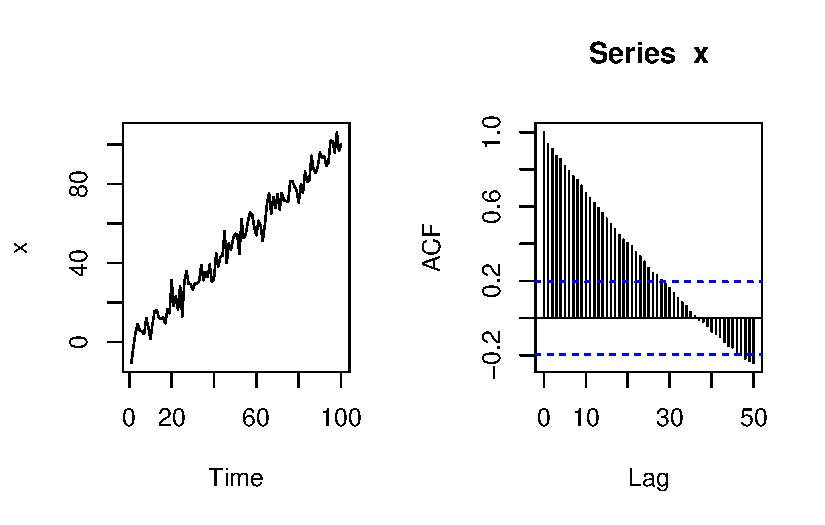
\includegraphics{polinomial_files/figure-pdf/unnamed-chunk-2-1.pdf}

\begin{Shaded}
\begin{Highlighting}[]
\FunctionTok{acf}\NormalTok{(Nile, }\AttributeTok{lwd =} \DecValTok{2}\NormalTok{)}
\end{Highlighting}
\end{Shaded}

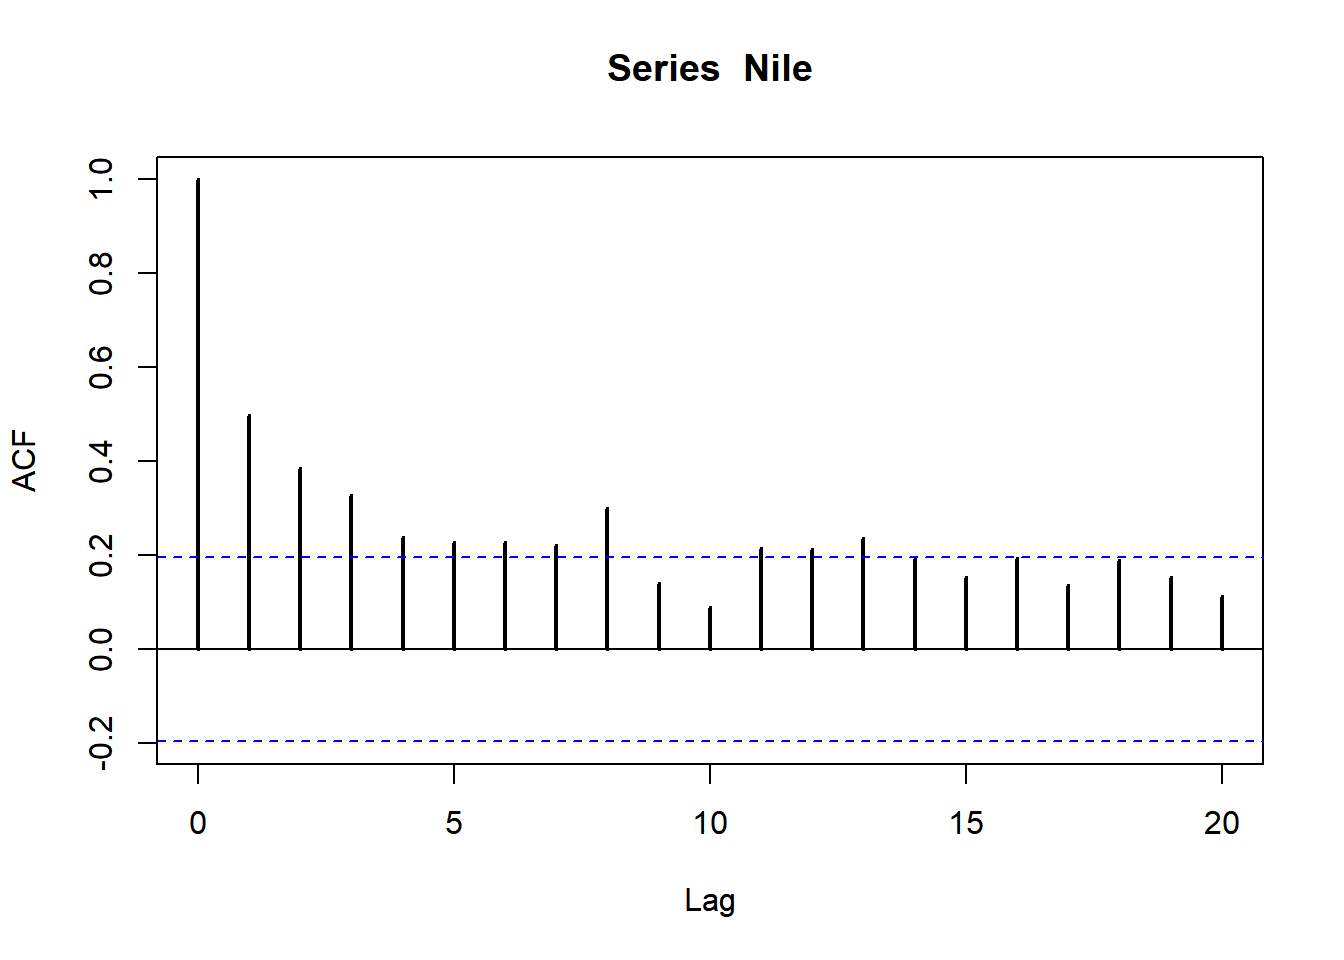
\includegraphics{polinomial_files/figure-pdf/unnamed-chunk-2-2.pdf}

É possível notar que há autocorrelação na série, mas o correlograma não
revela uma tendência forte. Abaixo mostramos a tendência estimada via
\texttt{loess}.

\begin{Shaded}
\begin{Highlighting}[]
\NormalTok{tempo }\OtherTok{\textless{}{-}} \DecValTok{1}\SpecialCharTok{:}\FunctionTok{length}\NormalTok{(Nile)}
\NormalTok{lw }\OtherTok{\textless{}{-}} \FunctionTok{loess}\NormalTok{( Nile }\SpecialCharTok{\textasciitilde{}}\NormalTok{ tempo)}
\NormalTok{tend }\OtherTok{\textless{}{-}} \FunctionTok{ts}\NormalTok{(lw}\SpecialCharTok{$}\NormalTok{fitted, }\AttributeTok{start =} \FunctionTok{start}\NormalTok{(Nile))}

\FunctionTok{ts.plot}\NormalTok{(Nile)}
\FunctionTok{lines}\NormalTok{(tend, }\AttributeTok{lwd =} \DecValTok{2}\NormalTok{, }\AttributeTok{col =} \StringTok{\textquotesingle{}tomato\textquotesingle{}}\NormalTok{)}
\end{Highlighting}
\end{Shaded}

\includegraphics{polinomial_files/figure-pdf/unnamed-chunk-3-1.pdf}

A tendência estimada via \texttt{loess} parece revelar um comportamento
inicial de queda e depois meio século de valores oscilando em torno de
do nível. Vamos analisar isso utilizando um modelo linear dinâmico para
o nível.

Primeiro, vamos criar um objeto que possui os componentes \(F\) e \(G\)
adequados. Para tanto, basta usar a função \texttt{dlmPoly} e escolher a
ordem do modelo polinomial.

\begin{Shaded}
\begin{Highlighting}[]
\FunctionTok{library}\NormalTok{(dlm)}
\NormalTok{mod }\OtherTok{\textless{}{-}} \FunctionTok{dlmModPoly}\NormalTok{( }\AttributeTok{order =} \DecValTok{1}\NormalTok{)}
\end{Highlighting}
\end{Shaded}

Se você tiver curiosidade, \(F\) e \(G\) estão guardados em lista, com
os nomes \texttt{FF} e \texttt{GG}

Dentro do objeto \texttt{mod} há um componente denomina \texttt{m0}. Ele
é a estimativa do nível antes de 1. Vamos simplesmente dizer que este é
igual ao valor observado em 1900

\begin{Shaded}
\begin{Highlighting}[]
\NormalTok{mod}\SpecialCharTok{$}\NormalTok{m0 }\OtherTok{\textless{}{-}}\NormalTok{ Nile[}\DecValTok{1}\NormalTok{]}
\end{Highlighting}
\end{Shaded}

Agora, vamos estimar as variâncias do modelo, para obter \(V\) e \(W\):

\begin{Shaded}
\begin{Highlighting}[]
\NormalTok{mod }\OtherTok{\textless{}{-}} \FunctionTok{modFim}\NormalTok{( Nile, mod)}
\end{Highlighting}
\end{Shaded}

Agora, vamos aplicar o Teorema de Bayes, através de uma série de
atualizações conhecidas como Filtro de Kalman

\begin{Shaded}
\begin{Highlighting}[]
\NormalTok{filtro }\OtherTok{\textless{}{-}} \FunctionTok{dlmFilter}\NormalTok{(Nile, mod)}
\end{Highlighting}
\end{Shaded}

Em modelos lineares dinâmicos, definimos o erro de previsão por

\[y_t-E(y_t|D_{t-1})=y_t-f_t.\] Se todos os sinais foram bem ajustados,
os erros de previsão possuem comportamento com um ruído branco. O valor
de \(f_t\) está no objeto \texttt{filtro}.

\begin{Shaded}
\begin{Highlighting}[]
\NormalTok{erro }\OtherTok{\textless{}{-}}\NormalTok{ Nile }\SpecialCharTok{{-}}\NormalTok{ filtro}\SpecialCharTok{$}\NormalTok{f}
\FunctionTok{ts.plot}\NormalTok{(erro)}
\end{Highlighting}
\end{Shaded}

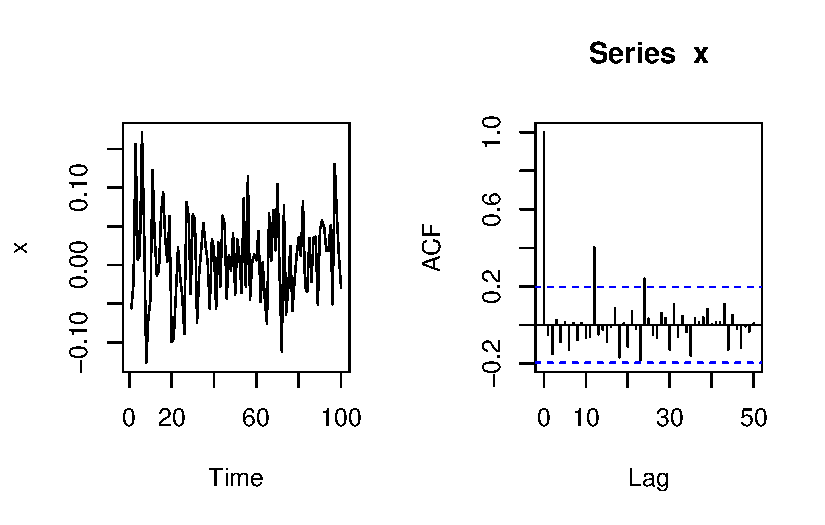
\includegraphics{polinomial_files/figure-pdf/unnamed-chunk-8-1.pdf}

\begin{Shaded}
\begin{Highlighting}[]
\FunctionTok{acf}\NormalTok{(erro)}
\end{Highlighting}
\end{Shaded}

\includegraphics{polinomial_files/figure-pdf/unnamed-chunk-8-2.pdf}

Agora, vamos reaplicar o Teorema de Bayes, considerando a amostra toda,
para obter a estimativa suavizada do nível.

\begin{Shaded}
\begin{Highlighting}[]
\NormalTok{suave }\OtherTok{\textless{}{-}} \FunctionTok{dlmSmooth}\NormalTok{(filtro)}

\FunctionTok{ts.plot}\NormalTok{(Nile)}
\FunctionTok{lines}\NormalTok{( suave}\SpecialCharTok{$}\NormalTok{s, }\AttributeTok{lwd =} \DecValTok{2}\NormalTok{, }\AttributeTok{col =} \StringTok{\textquotesingle{}seagreen\textquotesingle{}}\NormalTok{)}
\end{Highlighting}
\end{Shaded}

\includegraphics{polinomial_files/figure-pdf/unnamed-chunk-9-1.pdf}

Também podemos fazer um intervalo de credibidade para o nível suavizado.

\begin{Shaded}
\begin{Highlighting}[]
\FunctionTok{ts.plot}\NormalTok{(Nile)}
\FunctionTok{lines}\NormalTok{( suave}\SpecialCharTok{$}\NormalTok{s, }\AttributeTok{lwd =} \DecValTok{2}\NormalTok{, }\AttributeTok{col =} \StringTok{\textquotesingle{}seagreen\textquotesingle{}}\NormalTok{)}

\CommentTok{\# variâncias da suavização}
\NormalTok{vs }\OtherTok{\textless{}{-}} \FunctionTok{dlmSvd2var}\NormalTok{(suave}\SpecialCharTok{$}\NormalTok{U.S, suave}\SpecialCharTok{$}\NormalTok{D.S)}

\CommentTok{\# intervalo de credibilidade}
\FunctionTok{lines}\NormalTok{( suave}\SpecialCharTok{$}\NormalTok{s }\SpecialCharTok{{-}} \FloatTok{1.96}\SpecialCharTok{*}\FunctionTok{sqrt}\NormalTok{(}\FunctionTok{unlist}\NormalTok{(vs)) )}
\FunctionTok{lines}\NormalTok{( suave}\SpecialCharTok{$}\NormalTok{s }\SpecialCharTok{+} \FloatTok{1.96}\SpecialCharTok{*}\FunctionTok{sqrt}\NormalTok{(}\FunctionTok{unlist}\NormalTok{(vs)) )}
\end{Highlighting}
\end{Shaded}

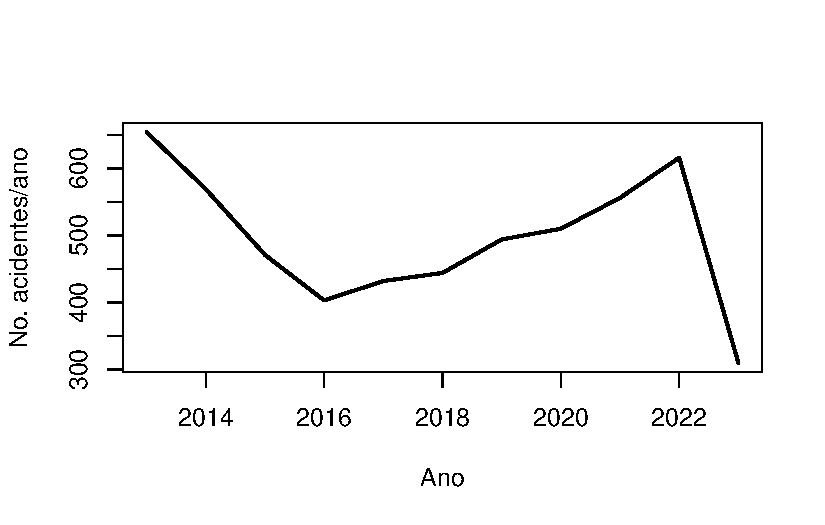
\includegraphics{polinomial_files/figure-pdf/unnamed-chunk-10-1.pdf}

Podemos fazer previsões com a função

\begin{Shaded}
\begin{Highlighting}[]
\NormalTok{prev }\OtherTok{\textless{}{-}} \FunctionTok{dlmForecast}\NormalTok{(filtro, }\DecValTok{3}\NormalTok{)}
\NormalTok{prev}\SpecialCharTok{$}\NormalTok{f}
\end{Highlighting}
\end{Shaded}

\begin{verbatim}
Time Series:
Start = 2000 
End = 2002 
Frequency = 1 
     Series 1
[1,] 782.6798
[2,] 782.6798
[3,] 782.6798
\end{verbatim}

\section{O modelo de tendência}\label{o-modelo-de-tenduxeancia}

O modelo linear dinâmico polinomial de segunda ordem é um modelo de
tendência, uma vez que sua função de previsão é

\[f_t(h)=m_{1,t}+m_{2,t}h.\]

Aqui, existem dois estados para cada tempo: \(\theta_{1,t}\) e
\(\theta_{2,t}\). No tempo \(t\), a média a posteriori dos estados
possui a seguinte interpretação:

\begin{itemize}
\item
  \(m_{1,t}\): é o nível (média) da série no tempo \(t\), estimado com
  todos os dados disponíveis até o tempo \(t\)
\item
  \(m_{2,t}:\) é a inclinação da tendência da série no tempo \(t\),
  estimado com todos os dados disponíveis até o tempo \(t\). Em
  particular, \(m_{2,t}>0\) indica tendência de crescimento, enquanto
  que \(m_{2,t}<0\) indica decrescimento.
\end{itemize}

Voltemos à série de acidentes aéreos mensais. `

\begin{Shaded}
\begin{Highlighting}[]
\FunctionTok{ts.plot}\NormalTok{(fab\_mes, }\AttributeTok{ylab =} \StringTok{\textquotesingle{}No acidentes/mês\textquotesingle{}}\NormalTok{)}
\end{Highlighting}
\end{Shaded}

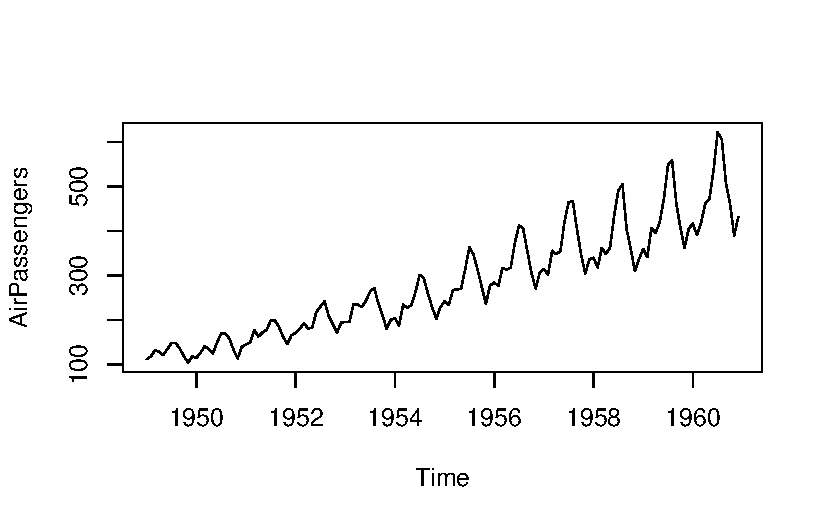
\includegraphics{polinomial_files/figure-pdf/unnamed-chunk-13-1.pdf}

\begin{Shaded}
\begin{Highlighting}[]
\FunctionTok{acf}\NormalTok{(fab\_mes, }\AttributeTok{main=}\StringTok{\textquotesingle{}\textquotesingle{}}\NormalTok{)}
\end{Highlighting}
\end{Shaded}

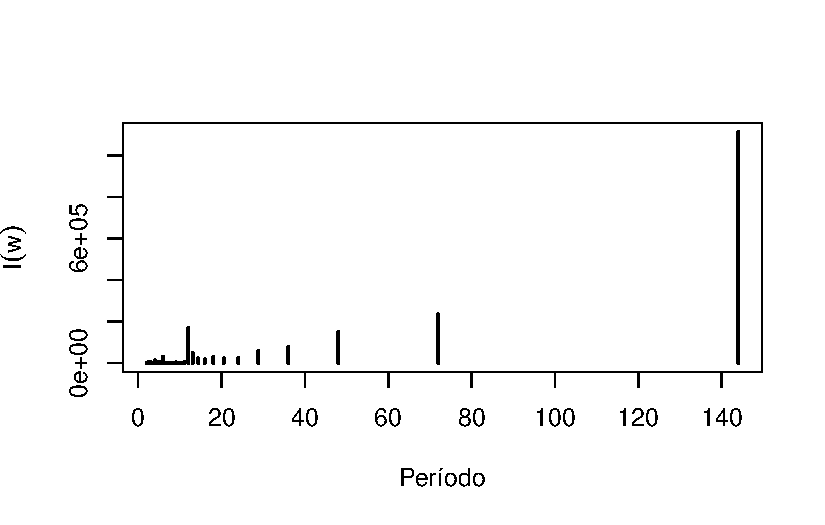
\includegraphics{polinomial_files/figure-pdf/unnamed-chunk-13-2.pdf}

Vamos construir um modelo linear para a tendência:

\begin{Shaded}
\begin{Highlighting}[]
\FunctionTok{require}\NormalTok{(dlm)}
\NormalTok{mod }\OtherTok{\textless{}{-}} \FunctionTok{dlmModPoly}\NormalTok{(}\DecValTok{2}\NormalTok{)}
\end{Highlighting}
\end{Shaded}

Em seguida, precisamos dar uma informação inicial sobre os estados no
tempo \(0\) (ou seja, a média do nível e da tendência antes da série ser
observada). Um bom começo é supor que \(m_{1,0}\) é o valor \(y_1\) - o
primeiro valor observado. Além disso, é usual iniciar a análise supondo
que a tendência é nula.

\begin{Shaded}
\begin{Highlighting}[]
\NormalTok{mod}\SpecialCharTok{$}\NormalTok{m0 }\OtherTok{\textless{}{-}} \FunctionTok{c}\NormalTok{(fab\_mes[}\DecValTok{1}\NormalTok{],}\DecValTok{0}\NormalTok{)}
\end{Highlighting}
\end{Shaded}

Agora, vamos estimar a variâncias do modelo:

\begin{Shaded}
\begin{Highlighting}[]
\NormalTok{mod }\OtherTok{\textless{}{-}} \FunctionTok{modFim}\NormalTok{(fab\_mes, mod)}
\end{Highlighting}
\end{Shaded}

Vamos estimar os parâmetros dos estados via filtro de Kalman.

\begin{Shaded}
\begin{Highlighting}[]
\NormalTok{filtro }\OtherTok{\textless{}{-}} \FunctionTok{dlmFilter}\NormalTok{(fab\_mes, mod)}
\end{Highlighting}
\end{Shaded}

Vamos analisar os erros de previsão.

\begin{Shaded}
\begin{Highlighting}[]
\NormalTok{erros }\OtherTok{\textless{}{-}}\NormalTok{ fab\_mes }\SpecialCharTok{{-}}\NormalTok{ filtro}\SpecialCharTok{$}\NormalTok{f}
\FunctionTok{ts.plot}\NormalTok{(erros)}
\end{Highlighting}
\end{Shaded}

\includegraphics{polinomial_files/figure-pdf/unnamed-chunk-18-1.pdf}

\begin{Shaded}
\begin{Highlighting}[]
\FunctionTok{acf}\NormalTok{(erros)}
\end{Highlighting}
\end{Shaded}

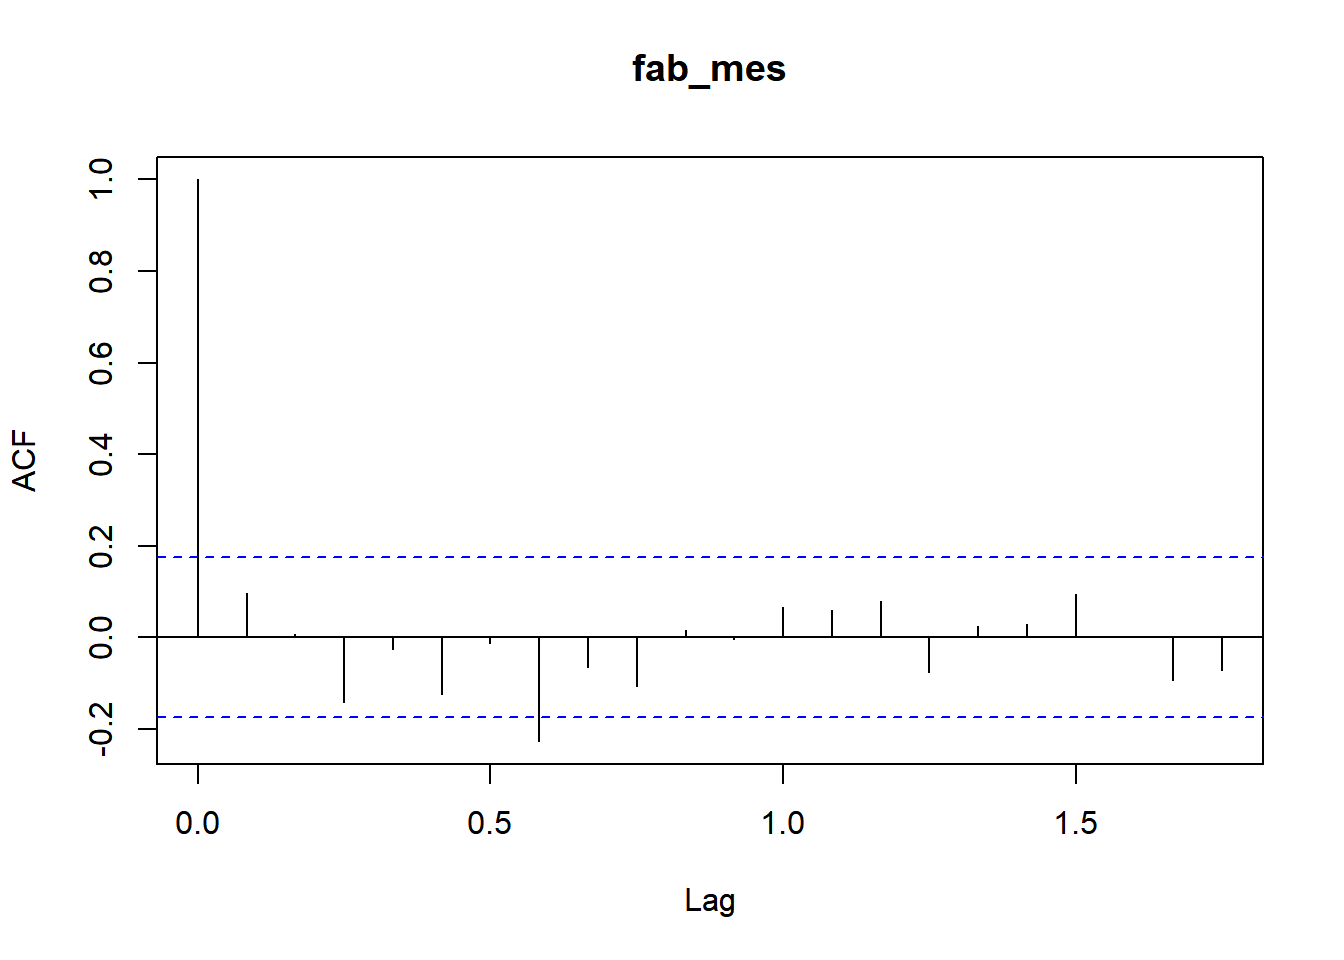
\includegraphics{polinomial_files/figure-pdf/unnamed-chunk-18-2.pdf}

Ambos os gráficos acima mostram um comportamento de ruído branco.

Podemos fazer previsões mais longas com este modelo. Abaixo vamos prever
o número de acidentes para os próximos 12 meses.

\begin{Shaded}
\begin{Highlighting}[]
\NormalTok{previsao12 }\OtherTok{\textless{}{-}} \FunctionTok{dlmForecast}\NormalTok{(filtro,}\DecValTok{12}\NormalTok{)}
\NormalTok{previsao12}\SpecialCharTok{$}\NormalTok{f}
\end{Highlighting}
\end{Shaded}

\begin{verbatim}
          Jan      Feb      Mar      Apr      May      Jun      Jul      Aug
2023                                                       51.70796 51.72957
2024 51.83762 51.85924 51.88085 51.90246 51.92407 51.94568                  
          Sep      Oct      Nov      Dec
2023 51.75118 51.77279 51.79440 51.81601
2024                                    
\end{verbatim}

Vamos colocar essas informações em um gráfico. Vamos começar com as
previsões um passo a frente, que são utilizadas para o cálculo do erro
de previsão e queforam realizadas dentro do filtro de Kalman - notem que
vamos começar as previsões em março, uma vez que as outras foram
irreais). Em seguida, vamos apresentar as previsões com um intervalo de
90\% de predição (não se usa 95\% para previsões porque os intervalos em
geral são grandes demais)

\begin{Shaded}
\begin{Highlighting}[]
\FunctionTok{ts.plot}\NormalTok{(fab\_mes,}\AttributeTok{xlim=}\FunctionTok{c}\NormalTok{(}\DecValTok{2013}\NormalTok{,}\DecValTok{2025}\NormalTok{), }\AttributeTok{ylab=}\StringTok{\textquotesingle{}No. acidentes mensais\textquotesingle{}}\NormalTok{, }\AttributeTok{ylim=}\FunctionTok{c}\NormalTok{(}\DecValTok{0}\NormalTok{,}\DecValTok{75}\NormalTok{))}
\FunctionTok{lines}\NormalTok{( }\FunctionTok{window}\NormalTok{(filtro}\SpecialCharTok{$}\NormalTok{f,}\AttributeTok{start=}\FunctionTok{c}\NormalTok{(}\DecValTok{2013}\NormalTok{,}\DecValTok{3}\NormalTok{)), }\AttributeTok{lty=}\DecValTok{2}\NormalTok{,}\AttributeTok{lwd =} \DecValTok{2}\NormalTok{)}

\CommentTok{\# medidas para o intervalo de previsão}
\NormalTok{media\_prev }\OtherTok{\textless{}{-}}\NormalTok{ previsao12}\SpecialCharTok{$}\NormalTok{f}
\NormalTok{media\_prev }\OtherTok{\textless{}{-}} \FunctionTok{ts}\NormalTok{(media\_prev, }\AttributeTok{start =} \FunctionTok{c}\NormalTok{(}\DecValTok{2023}\NormalTok{,}\DecValTok{7}\NormalTok{), }\AttributeTok{frequency =} \DecValTok{12}\NormalTok{)}

\NormalTok{desv\_prev }\OtherTok{\textless{}{-}} \FunctionTok{sqrt}\NormalTok{( }\FunctionTok{unlist}\NormalTok{( previsao12}\SpecialCharTok{$}\NormalTok{Q))}
\NormalTok{desv\_prev }\OtherTok{\textless{}{-}} \FunctionTok{ts}\NormalTok{(desv\_prev, }\AttributeTok{start =} \FunctionTok{c}\NormalTok{(}\DecValTok{2023}\NormalTok{,}\DecValTok{7}\NormalTok{), }\AttributeTok{frequency =} \DecValTok{12}\NormalTok{)}

\CommentTok{\# intervalo de 90\% para as previsões}
\FunctionTok{lines}\NormalTok{(media\_prev, }\AttributeTok{lwd =} \DecValTok{2}\NormalTok{, }\AttributeTok{col =}\StringTok{\textquotesingle{}blue\textquotesingle{}}\NormalTok{)}
\FunctionTok{lines}\NormalTok{(media\_prev }\SpecialCharTok{{-}}\FloatTok{1.64}\SpecialCharTok{*}\NormalTok{desv\_prev, }\AttributeTok{lwd =} \DecValTok{2}\NormalTok{, }\AttributeTok{col =}\StringTok{\textquotesingle{}blue\textquotesingle{}}\NormalTok{)}
\FunctionTok{lines}\NormalTok{(media\_prev}\FloatTok{+1.64}\SpecialCharTok{*}\NormalTok{desv\_prev, }\AttributeTok{lwd =} \DecValTok{2}\NormalTok{, }\AttributeTok{col =}\StringTok{\textquotesingle{}blue\textquotesingle{}}\NormalTok{)}

\CommentTok{\# legenda}
\FunctionTok{legend}\NormalTok{(}\StringTok{\textquotesingle{}bottomleft\textquotesingle{}}\NormalTok{,}\FunctionTok{c}\NormalTok{(}\StringTok{\textquotesingle{}Série observada\textquotesingle{}}\NormalTok{,}\StringTok{\textquotesingle{}Previsão 1 passo à frente\textquotesingle{}}\NormalTok{, }\StringTok{\textquotesingle{}Previsão de 12 meses\textquotesingle{}}\NormalTok{), }\AttributeTok{lty=}\FunctionTok{c}\NormalTok{(}\DecValTok{1}\NormalTok{,}\DecValTok{2}\NormalTok{,}\DecValTok{1}\NormalTok{), }\AttributeTok{col =}\FunctionTok{c}\NormalTok{(}\DecValTok{1}\NormalTok{,}\DecValTok{1}\NormalTok{,}\StringTok{\textquotesingle{}blue\textquotesingle{}}\NormalTok{), }\AttributeTok{bty =} \StringTok{\textquotesingle{}n\textquotesingle{}}\NormalTok{)}
\end{Highlighting}
\end{Shaded}

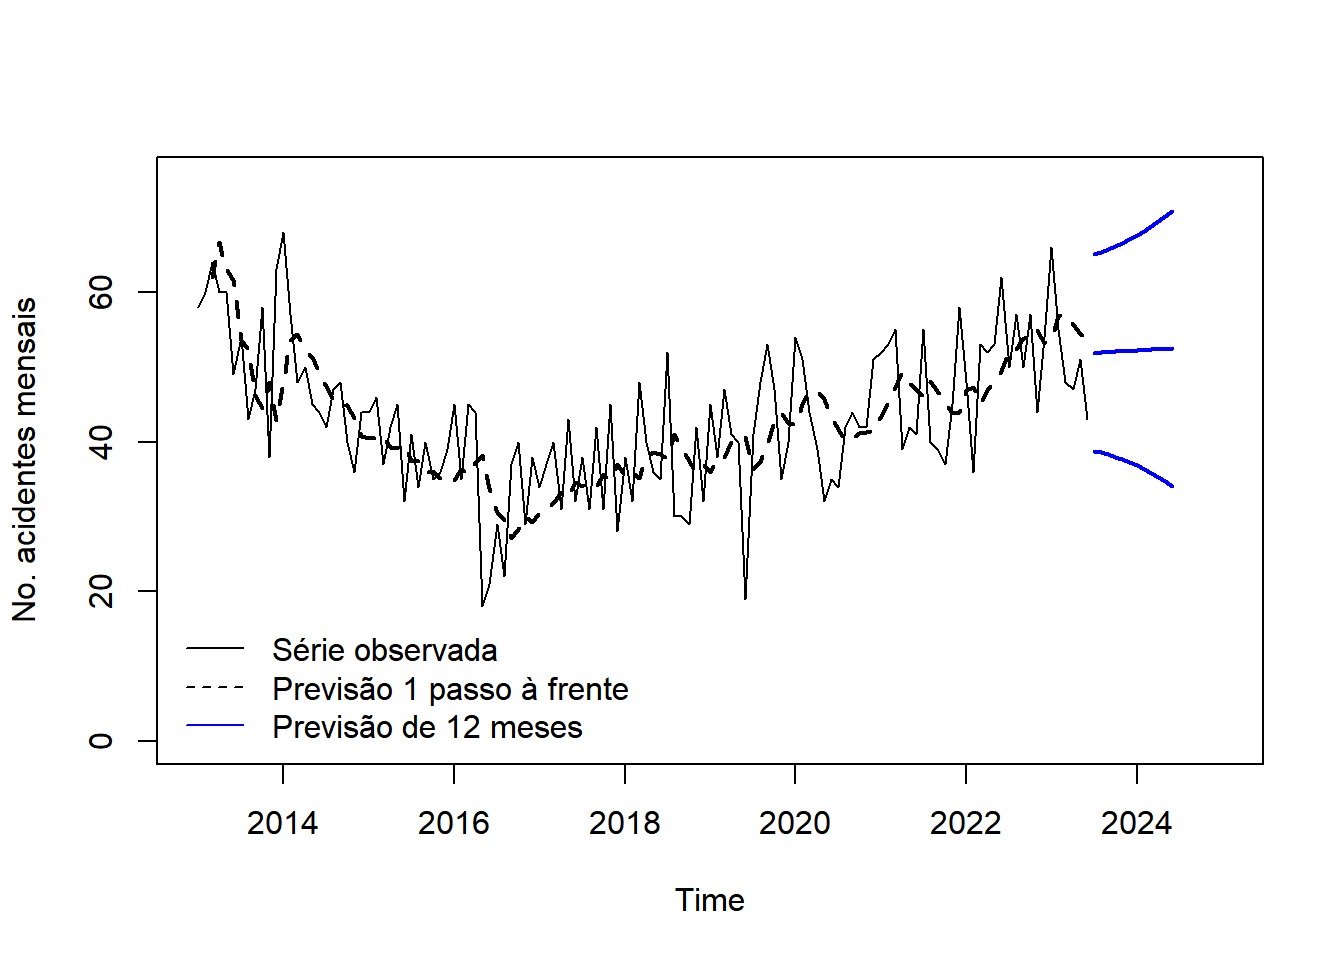
\includegraphics{polinomial_files/figure-pdf/unnamed-chunk-20-1.pdf}

Agora vamos estudar os estados suavizados. `

\begin{Shaded}
\begin{Highlighting}[]
\NormalTok{suave }\OtherTok{\textless{}{-}} \FunctionTok{dlmSmooth}\NormalTok{(filtro)}
\end{Highlighting}
\end{Shaded}

A obtenção das variâncias é mais delicada. Em cada instante de tempo, é
calculada a matriz

\[S_t=\left( \begin{array}{cc} s_{11,t} & s_{12,t}\\s_{12,t}&s_{22,t}\end{array}\right),\]
que reprenta em sua diagonal a variância dos estados e fora dela a
covariância entre eles. Por motivos computacionais, a matriz \(S_t\) não
é computada diretamente, mas sim duas matrizes \(U_t\) e \(D_t\) tais
que

\[S_t=U_t D_t U_t'\] Essa decomposição, conhecida como espectral, possui
vantagens numéricas que facilitam o processo de inversão necessário no
filtro de Kalman. A função abaixo recupera o desvio padrão a partir de
\(U_t\) e \(D_t\).

\begin{Shaded}
\begin{Highlighting}[]
\NormalTok{sdSmooth }\OtherTok{\textless{}{-}} \ControlFlowTok{function}\NormalTok{(suave)\{}
\NormalTok{  n }\OtherTok{\textless{}{-}} \FunctionTok{nrow}\NormalTok{(suave}\SpecialCharTok{$}\NormalTok{s)}
\NormalTok{  q }\OtherTok{\textless{}{-}} \FunctionTok{ncol}\NormalTok{(suave}\SpecialCharTok{$}\NormalTok{s)}
\NormalTok{  dp }\OtherTok{\textless{}{-}} \FunctionTok{array}\NormalTok{(}\ConstantTok{NA\_real\_}\NormalTok{, }\FunctionTok{c}\NormalTok{( n , q))}
  \ControlFlowTok{for}\NormalTok{(i }\ControlFlowTok{in} \DecValTok{1}\SpecialCharTok{:}\NormalTok{n)\{}
\NormalTok{    S }\OtherTok{\textless{}{-}} \FunctionTok{dlmSvd2var}\NormalTok{(suave}\SpecialCharTok{$}\NormalTok{U.S[[i]],suave}\SpecialCharTok{$}\NormalTok{D.S[i,])}
\NormalTok{    dp[i,] }\OtherTok{\textless{}{-}} \FunctionTok{sqrt}\NormalTok{( }\FunctionTok{diag}\NormalTok{(S))}
\NormalTok{  \}}
\NormalTok{  dp}
\NormalTok{\}}
\end{Highlighting}
\end{Shaded}

Abaixo, vamos obter os desvios da suavização

\begin{Shaded}
\begin{Highlighting}[]
\NormalTok{sd }\OtherTok{\textless{}{-}} \FunctionTok{sdSmooth}\NormalTok{(suave)}
\end{Highlighting}
\end{Shaded}

Vamos começar a análise com o nível. Observe que, como são 2 estados,
devemos selecionar a coluna 1.

\begin{Shaded}
\begin{Highlighting}[]
\NormalTok{nivel\_medio }\OtherTok{\textless{}{-}}\NormalTok{ suave}\SpecialCharTok{$}\NormalTok{s[,}\DecValTok{1}\NormalTok{]}
\NormalTok{sd\_nivel }\OtherTok{\textless{}{-}}\NormalTok{ sd[,}\DecValTok{1}\NormalTok{]}

\FunctionTok{ts.plot}\NormalTok{(fab\_mes)}
\FunctionTok{lines}\NormalTok{(nivel\_medio, }\AttributeTok{lwd =} \DecValTok{2}\NormalTok{, }\AttributeTok{col =} \StringTok{\textquotesingle{}seagreen\textquotesingle{}}\NormalTok{)}

\CommentTok{\# intervalor de credibilidade (95\%) para o nível}
\FunctionTok{lines}\NormalTok{(nivel\_medio }\SpecialCharTok{{-}} \FloatTok{1.96}\SpecialCharTok{*}\NormalTok{sd\_nivel, }\AttributeTok{lwd =} \DecValTok{2}\NormalTok{, }\AttributeTok{col =} \StringTok{\textquotesingle{}seagreen\textquotesingle{}}\NormalTok{, }\AttributeTok{lty=} \DecValTok{2}\NormalTok{)}
\FunctionTok{lines}\NormalTok{(nivel\_medio }\SpecialCharTok{+} \FloatTok{1.96}\SpecialCharTok{*}\NormalTok{sd\_nivel, }\AttributeTok{lwd =} \DecValTok{2}\NormalTok{, }\AttributeTok{col =} \StringTok{\textquotesingle{}seagreen\textquotesingle{}}\NormalTok{, }\AttributeTok{lty=}\DecValTok{2}\NormalTok{)}
\end{Highlighting}
\end{Shaded}

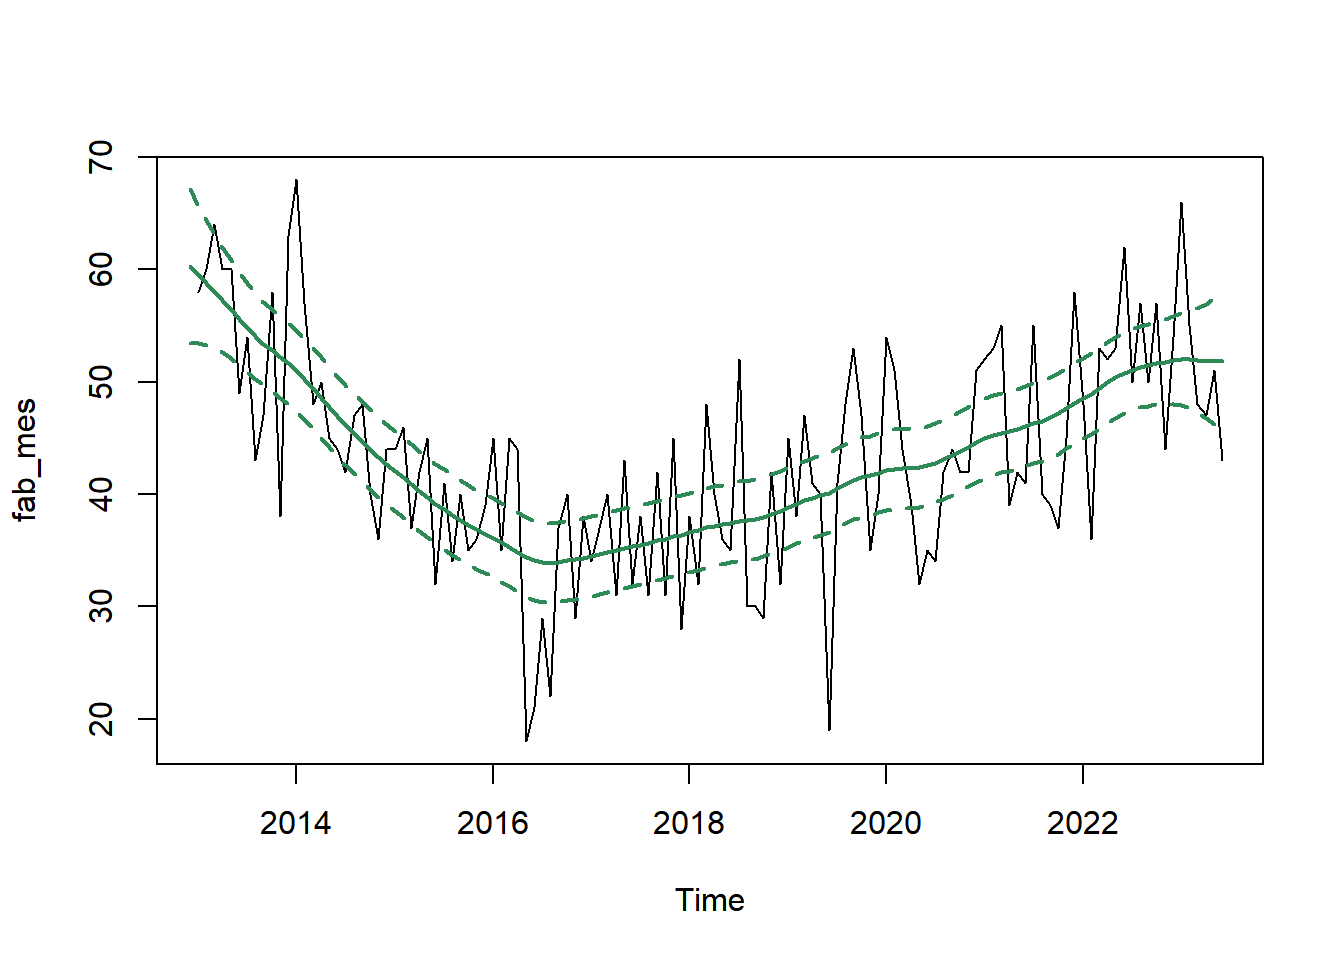
\includegraphics{polinomial_files/figure-pdf/unnamed-chunk-24-1.pdf}

Por último, vamos analisar a inclinação da tendência. Como a média da
série já foi modelada pelo nível, os gráficos das demais componentes não
são colocados sobre a série original. Abaixo mostramos o gráfico da
inclinação, com seu respectivo intervalo.

\begin{Shaded}
\begin{Highlighting}[]
\NormalTok{tend }\OtherTok{\textless{}{-}}\NormalTok{ suave}\SpecialCharTok{$}\NormalTok{s[,}\DecValTok{2}\NormalTok{]}
\NormalTok{sd\_tend }\OtherTok{\textless{}{-}}\NormalTok{ sd[,}\DecValTok{2}\NormalTok{]}
\FunctionTok{ts.plot}\NormalTok{(tend, }\AttributeTok{lwd =} \DecValTok{2}\NormalTok{, }\AttributeTok{ylim=}\FunctionTok{c}\NormalTok{(}\SpecialCharTok{{-}}\FloatTok{1.5}\NormalTok{,}\DecValTok{1}\NormalTok{), }\AttributeTok{ylab=}\StringTok{\textquotesingle{}Inclinação da tendência\textquotesingle{}}\NormalTok{)}
\FunctionTok{lines}\NormalTok{(tend}\FloatTok{{-}1.96}\SpecialCharTok{*}\NormalTok{sd\_tend)}
\FunctionTok{lines}\NormalTok{(tend}\FloatTok{+1.96}\SpecialCharTok{*}\NormalTok{sd\_tend)}
\FunctionTok{abline}\NormalTok{(}\AttributeTok{h=}\DecValTok{0}\NormalTok{, }\AttributeTok{lty =} \DecValTok{2}\NormalTok{)}

\CommentTok{\# período de mudança da tendência de decrescente para crescente}
\FunctionTok{abline}\NormalTok{(}\AttributeTok{v=}\DecValTok{2016}\SpecialCharTok{+}\DecValTok{10}\SpecialCharTok{/}\DecValTok{12}\NormalTok{, }\AttributeTok{lty =} \DecValTok{2}\NormalTok{)}
\FunctionTok{points}\NormalTok{(}\DecValTok{2016}\SpecialCharTok{+}\DecValTok{10}\SpecialCharTok{/}\DecValTok{12}\NormalTok{,}\DecValTok{0}\NormalTok{, }\AttributeTok{pch =} \DecValTok{15}\NormalTok{, }\AttributeTok{cex =} \FloatTok{1.2}\NormalTok{)}
\FunctionTok{text}\NormalTok{(}\DecValTok{2016}\SpecialCharTok{+}\DecValTok{11}\SpecialCharTok{/}\DecValTok{12}\NormalTok{,.}\DecValTok{1}\NormalTok{,}\StringTok{\textquotesingle{}Oct 16\textquotesingle{}}\NormalTok{, }\AttributeTok{pos =} \DecValTok{2}\NormalTok{)}

\CommentTok{\# identificando a desaceleração}
\NormalTok{x }\OtherTok{\textless{}{-}} \FunctionTok{window}\NormalTok{(tend, }\AttributeTok{start=}\FunctionTok{c}\NormalTok{(}\DecValTok{2022}\NormalTok{,}\DecValTok{7}\NormalTok{) )}
\FunctionTok{abline}\NormalTok{(}\AttributeTok{v=}\DecValTok{2022}\SpecialCharTok{+}\DecValTok{7}\SpecialCharTok{/}\DecValTok{12}\NormalTok{, }\AttributeTok{lty =} \DecValTok{2}\NormalTok{)}
\FunctionTok{points}\NormalTok{(}\DecValTok{2022}\SpecialCharTok{+}\DecValTok{7}\SpecialCharTok{/}\DecValTok{12}\NormalTok{, x[}\DecValTok{1}\NormalTok{], }\AttributeTok{pch =} \DecValTok{15}\NormalTok{, }\AttributeTok{cex =} \FloatTok{1.2}\NormalTok{)}
\FunctionTok{text}\NormalTok{(}\DecValTok{2022}\SpecialCharTok{+}\DecValTok{7}\SpecialCharTok{/}\DecValTok{12}\NormalTok{,x[}\DecValTok{1}\NormalTok{],}\StringTok{\textquotesingle{}Jul 22\textquotesingle{}}\NormalTok{, }\AttributeTok{pos =} \DecValTok{2}\NormalTok{)}
\end{Highlighting}
\end{Shaded}

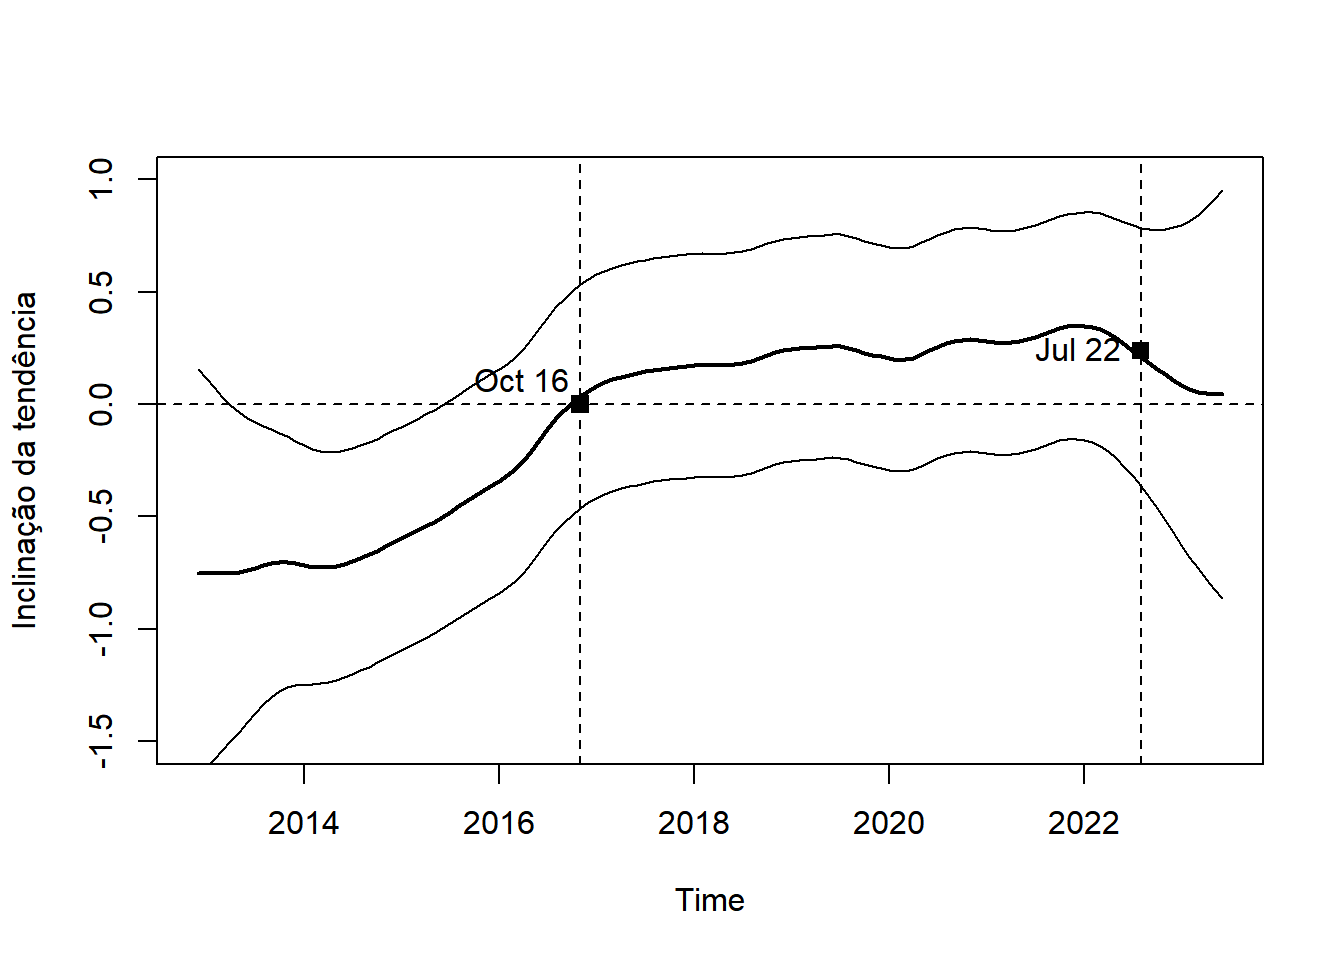
\includegraphics{polinomial_files/figure-pdf/unnamed-chunk-25-1.pdf}

Com o gráfico acima, identificamos muitas características interessantes.

\begin{itemize}
\item
  Note que o zero está presente na maior parte do intervalo. Portanto,
  podemos apenas afirmar que em certos períodos, a tendência de
  crescimento/decrescimento foram mais prováveis.
\item
  Em relação à inclinação média, podemos afirmar que existem evidências
  de que o padrão de decrescimento estava desacelerando antes de 2016,
  culminando na inflexão em outubro. Nesse período a série passou a ter
  uma taxa de crescimento relativamente constante até Julho de 2022,
  quando começou a desacelar.
\end{itemize}

\section{Exercícios}\label{exercuxedcios-1}

Abaixo, mostramos o número de homicídios mensais em Manaus entre Janeiro
de 1979 e Dezembro de 2009.

\begin{Shaded}
\begin{Highlighting}[]
\NormalTok{url }\OtherTok{\textless{}{-}} \StringTok{\textquotesingle{}https://www.dropbox.com/s/hcqq6uhgwnimpcn/homicidios\_manaus\_SIM.csv?dl=1\textquotesingle{}}
\end{Highlighting}
\end{Shaded}

\begin{itemize}
\item
  Explore a série.
\item
  Estude o nível da série
\item
  Estude o comportamento da inclinação, identificando possíveis regimes
  de aceleração/desaceleração de crescimento.
\end{itemize}

Analise a série de suicídios no Mato Grosso do Sul, estudando o nível da
série e a inclinação da tendência.

\begin{Shaded}
\begin{Highlighting}[]
\NormalTok{url }\OtherTok{\textless{}{-}} \StringTok{\textquotesingle{}https://drive.google.com/uc?authuser=0\&id=1DMSgrQDl0636Lw0Y0MYJHJrgw\_2uXntM\&export=download\textquotesingle{}}
\end{Highlighting}
\end{Shaded}

\bookmarksetup{startatroot}

\chapter*{References}\label{references}
\addcontentsline{toc}{chapter}{References}

\markboth{References}{References}

\phantomsection\label{refs}
\begin{CSLReferences}{0}{1}
\end{CSLReferences}




\end{document}
